\documentclass[11pt]{article}

\def\articlename{统计整理}
\def\authorname{杨弘毅}
\def\startdate{2020年4月9日}

\ifx \authorname\undefined
  \def\authorname{杨弘毅}
\else
\fi

\author{\authorname}
\date{创建:\startdate \\修改:\today}

\usepackage[a4paper,left=6em,right=6em]{geometry}
\usepackage{amsmath,amsfonts,amsthm,bbold}
\usepackage{booktabs,float,multirow}
\usepackage{cancel}
\usepackage{enumitem}
\usepackage{multicol}
\usepackage{graphicx}
\usepackage[toc,title]{appendix}
\usepackage{tikz}
\usetikzlibrary{arrows.meta}
\usetikzlibrary{patterns}
\usetikzlibrary{decorations.pathreplacing}
\usetikzlibrary{decorations.pathmorphing}
\usepackage{subcaption}
\usepackage{fancyhdr}
\pagestyle{fancy}
\setlength{\headheight}{15pt}
\usepackage{footmisc}
\usepackage{hyperref}
\usepackage{tocloft}
\hypersetup{
    colorlinks=true, %set true if you want colored links
    linkcolor=blue,
    linktoc=all, %set to all if you want both sections and subsections linked
    citecolor=black,
    filecolor=black,
    urlcolor=blue
}
\usepackage[UTF8]{ctex}

\title{\articlename}

% Format
\setlength{\cftbeforesecskip}{6pt}
\setlength{\parskip}{0.6em}
\renewcommand{\baselinestretch}{1.4}
\setlist{noitemsep,itemindent=1em,topsep=0em,leftmargin=4em,rightmargin=4em}
\setlist[2]{leftmargin=2em}

% Shortcut
\newcommand{\divider}{\vspace{-\parskip}\noindent\rule{\linewidth}{0.4pt}}
\newcommand{\tops}[1]{\texorpdfstring{#1}{TEXT}}

% Theorem
\newtheorem{thm}{定理}[section] 
\newtheorem{proposition}[thm]{命题}
\newtheorem{lemma}[thm]{引理}
\newtheorem{corollary}[thm]{推论}
\newtheorem{property}[thm]{性质}
\newtheorem{example}[thm]{例子}
\newtheorem{remark}[thm]{备注}
\newtheorem{note}[thm]{注释}

% Symbol
\newcommand{\E}{\mathbb{E}}
\newcommand{\mcl}{\mathcal{L}}
\newcommand{\rnE}{\widetilde{\mathbb{E}}}
\newcommand{\wt}[1]{\widetilde{#1}}
\DeclareMathOperator{\Var}{Var}
\DeclareMathOperator{\Cov}{Cov}
\newcommand{\abs}[1]{\left\lvert #1\right\rvert}
\newcommand{\norm}[1]{\left\lVert #1\right\rVert}
\newcommand{\given}{\:\vert\:}

\begin{document}
\maketitle
\tableofcontents

\section{TODO}
\begin{itemize}
    \item exact test
    \item likelihood, log-likelihood, goodness-of-fit, quasi-maximum likelihood, ratio test
    \item Newey West 1987
\end{itemize}

\section{基础定义}

\subsection{期望}

对于随机变量$X$,其概率空间为$(\Omega,\mathcal{F},P)$,期望值$\E[X]$或$\mu$,应有:
\begin{equation*}
    \E[X] = \int_{\Omega} X(\omega) dP(\omega)
\end{equation*}

在离散以及连续情形下有如下定义,其中$f(x)$为变量$X$的概率密度函数(PDF)。
\begin{align*}
    \E[X] &= \sum_{i=i}^n x_i p_i =x_1 p_1 + x_2 p_2 + \dots + x_n p_n \\
    \E[X] &= \int x f(x) dx
\end{align*}

其性质有:
\begin{align*}
    \E[X+Y] &= \E[X] + \E[Y] \\
    \E[aX] &= a \E[X] \\
    \E[XY] &= \E[X]\E[Y] \quad \text{(X,Y are independent)}
\end{align*}

\subsection{方差}

对于方差(Variance)或$\sigma^2$,定义有:
\begin{align*}
    \Var(X) &= \E\left[ (X-\mu)^2 \right]\\
    &= \E[(X-\E[X])^2] \\
    &= \E[X^2 - 2X\E[X] + \E[X]^2] \\
    &= \E[X^2] - 2\E[X]^2 + \E[X]^2 \\
    &= \E[X^2] - \E[X]^2 \\
    &= \Cov(X,X)
\end{align*}

同理,或其连续积分形式有:
\begin{align*}
    \Var(X) &= \int (X-\mu)^2 f(x) dx \\
    &= \int x^2 f(x) dx - 2\mu \int xf(x)dx + \mu^2 \int f(x)dx \\
    &= \int x^2 f(x) dx - \mu^2
\end{align*}

其性质有:
\begin{align*}
    \Var(X + a) &= \Var(X) \\
    \Var(aX) &= a^2\Var(X) \\
    \Var(aX \pm bY) &= a^2\Var(X) + b^2\Var(Y) \pm 2ab \Cov(X,Y) \\
    \Var(\sum_{i=1}^{N} X_i) &= \sum_{i,j=1}^{N}\Cov(X_i,X_j) = \sum_{i=1}^{N}\Var(X_i) + \sum_{i \neq j}\Cov(X_i,X_j) \\
    \Var(\sum_{i=1}^{N} a_i X_i) &= \sum_{i,j=1}^{N}a_i a_j\Cov(X_i,X_j) \\
    &= \sum_{i=1}^{N}a_i^2\Var(X_i) + \sum_{i \neq j} a_i a_j \Cov(X_i,X_j) \\
    &= \sum_{i=1}^{N}a_i^2\Var(X_i) + 2\sum_{1 \leq i \leq j \leq N} a_i a_j \Cov(X_i,X_j)
\end{align*}

\subsection{协方差}

对于协方差(Covariance)其定义有:
\begin{align*}
    \Cov(X,Y) &= \E[(X-E(X))(Y-E(Y))] \\
    &= \E[XY - X\E[Y] -Y\E[X]+ \E[X]\E[Y]] \\
    &= \E[XY] - \E[X]\E[Y] - \E[X]\E[Y] + \E[X]\E[Y] \\
    &= \E[XY] - \E[X]\E[Y]
\end{align*}

性质有:
\begin{align*}
    \Cov(X,a) &= 0 \\
    \Cov(X,X) &= \Var(X) \\
    \Cov(X,Y) &= \Cov(Y,X) \\
    \Cov(aX,bY) &= ab\Cov(X,Y) \\
    \Cov(X+a,Y+b) &= \Cov(X,Y) \\
    \Cov(aX+bY,cW+dV) &= ac\Cov(X,W)+ad\Cov(X,V) \\
    &\hspace{2em} +bc\Cov(Y,W)+bd\Cov(Y,V)
\end{align*}

\subsection{相关系数}

相关系数(Correlation Coefficient),为研究变量间线性相关程度的量。最早由统计学家卡尔·皮尔逊设计,也称为皮尔逊积矩相关系数(Pearson product-moment correlation coefficient),或皮尔逊相关系数:
\begin{equation*}
    \rho_{X,Y} = \frac{\Cov(X,Y)}{\sigma_X\sigma_Y}
    = \frac{\E[(X-\E[X])(Y-\E[Y])]}{\sigma_X\sigma_Y}
\end{equation*}

\section{矩}

\subsection{理解}

在物理学中,矩(Moment)源于阿基米德的杠杆原理,可简单认为是物理量与参照点距离的乘积,如力与力臂(参考点的距离)的乘积,得到的是力矩(或扭矩)。如一杆“秤”,“秤”的平衡的两边重量与距离的乘积相同,则能保持平衡。

具体而言,$n$阶矩$\mu_n$为物理量$Q$与某参考点$x$的$n$次方的乘积,即$\mu_n = x^n Q$。常见的物理量如力或电荷等,若物理量并非集中在单点上,矩就应该是在物理量在空间上的积分,因有:$\mu_u = \int x^n f(x) dr$,其中$f(x)$为物理量的密度分布函数。

而物理中的矩与数学中的矩概念相通,而在概率论上,如一端秤砣重量为中奖金额$500$元,中奖概率为百分之一,即离中心点距离为$0.01$,那么其期望应为为$5$元。可以理解为了使得秤保持平衡,则另一端,在距离中心距离为$1$,对应其秤砣重量中奖金额应为$5$元。

\begin{figure}[ht!]
    \centering
    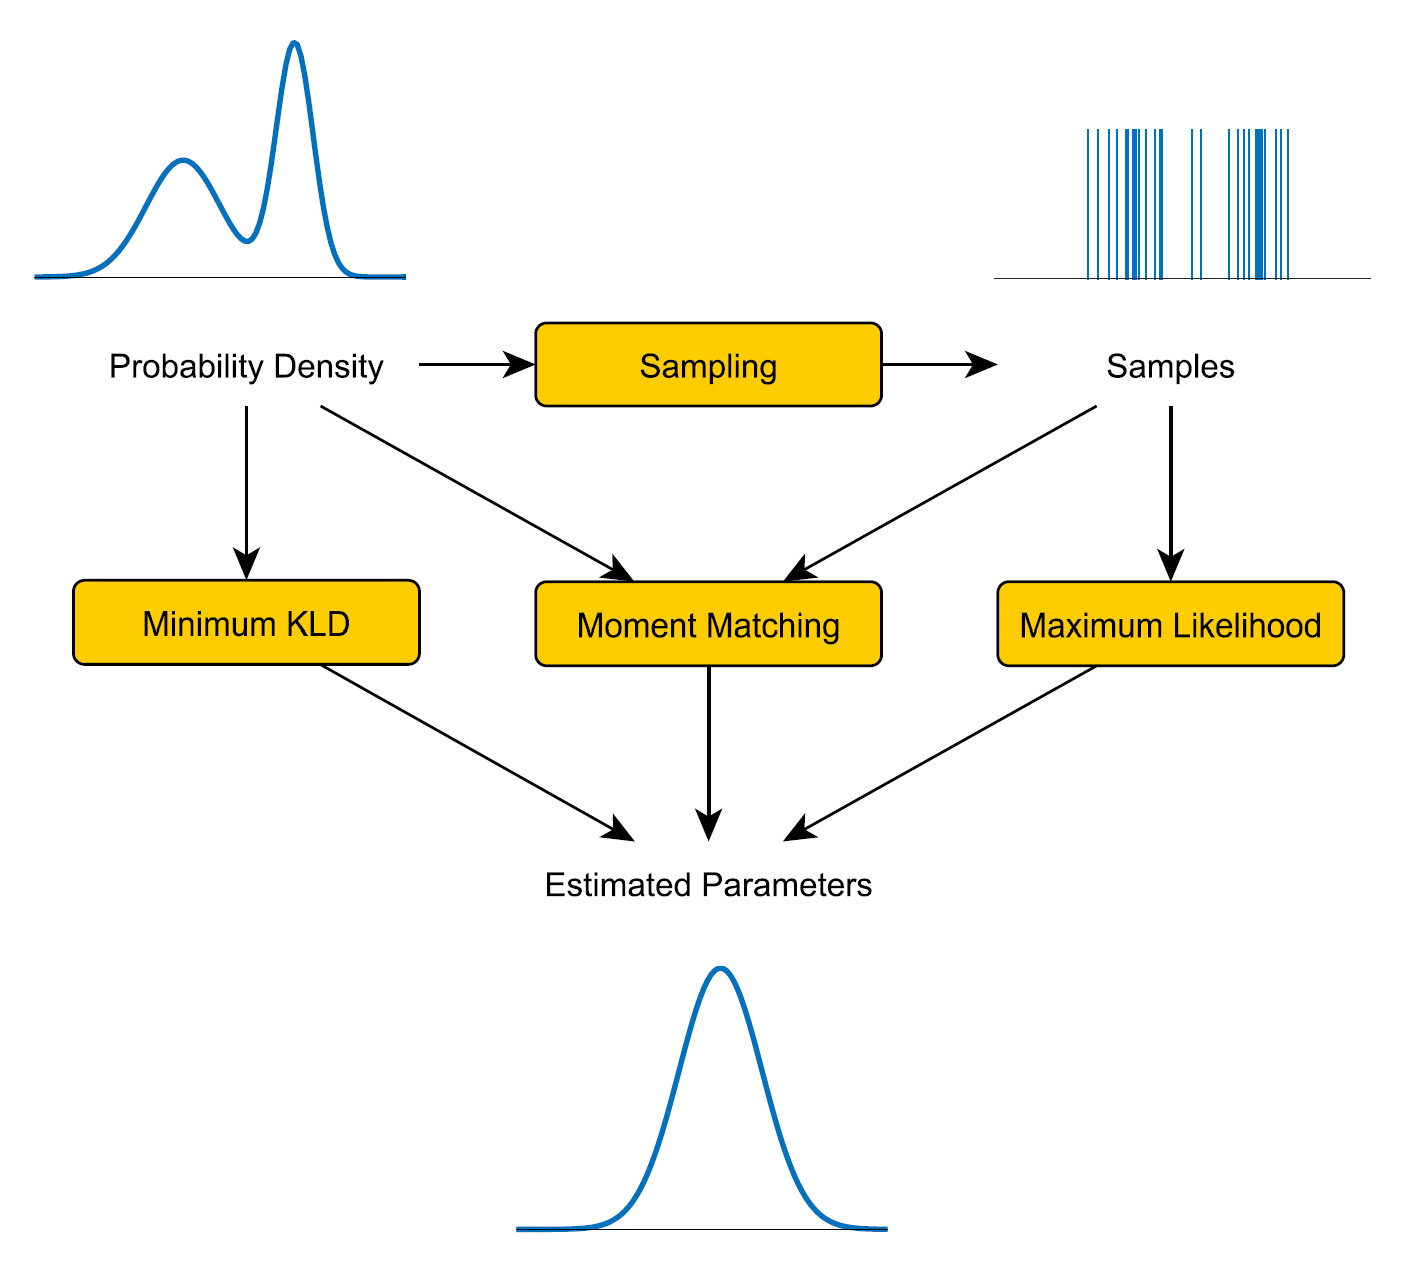
\includegraphics[width=0.6\textwidth]{fig/moment-matching.png}
    \caption{矩匹配}
    \label{fig:moment-match}
\end{figure}

\subsection{定义}

根据上述理解,物理学中与数学中的矩概念相通,即距离(概率)乘以物理量(随机变量)的大小。$p_i$为概率质量函数(Probability mass function,PMF),则对于n阶矩的离散形式有:
\begin{equation*}
    \E[x^n] = \sum_i x_i^n p_i
\end{equation*}

在连续形式下,n阶矩可以表示为$(x-c)^n$的期望,其中$f(x)$为概率密度函数(Probability density function,PDF),其中c为均值。当c为0时,即称为中心距(Central moment)。相反,则称为非中心矩,或原始矩(Raw moment):
\begin{equation*}
    \E[x^n] = \mu_n = \int_{-\infty}^{\infty} (x-c)^n f(x) dx
\end{equation*}

除了根据$c$是否为零,根据是否进行标准化处理,可细分为标准矩。常用的矩有:
\begin{itemize}
    \item 均值 $\text{Mean}(X)=\E(X)$ 为一阶非中心矩
    \item 方差 $\text{Variance}(X) = \E(X-\mu)^2$ 为二阶中心矩
    \item 偏度 $\text{Skewness}(X) = \frac{\E[(X-\mu)^4]}{\sigma^3}$ 为三阶标准矩 
    \item 峰度 $\text{Kurtosis}(X) = \frac{\E[(X-\mu)^4]}{\sigma^4}$ 为四阶标准矩
\end{itemize}

\subsection{分类}

根据如上定义,从零阶至四阶的原始矩与中心矩有如下定义,其中定义$\sigma = \left(\E[(X-\mu)^2]\right)^{\frac{1}{2}}$。正态分布由它的前两阶矩决定,而对于其他的分布,需要了解更高阶矩。同时注意到三阶矩以上都称标准矩,如同方差要去除均值的影响,偏度和峰度也要去除方差的影响。
\begin{table}[ht!]
\centering
\begin{tabular}{@{}clll@{}}
\toprule
\textbf{阶} & \multicolumn{1}{c}{\textbf{原始矩}} & \multicolumn{1}{c}{\textbf{中心矩}} & \multicolumn{1}{c}{\textbf{标准矩}} \\ \midrule
\textbf{0} & $\E(x^0)= 1 $ & $\E[(X-\mu)^0] = 1$ & $\frac{\E[(X-\mu)^0]}{\sigma^0} = 1$ \\
\textbf{1} & $\E(x^1)= \mu \,\text{(均值)} $ & $\E[(X-\mu)^1] = 0$ & $\frac{\E[(X-\mu)^1]}{\sigma^1} = 0$ \\
\textbf{2} & $\E(x^2) $ & $\E[(X-\mu)^2] = \sigma^2$ \,\text{(方差)} & $\frac{\E[(X-\mu)^2]}{\sigma^2} = 1$ \\
\textbf{3} & $\E(x^3) $ & $\E[(X-\mu)^3]$ & $\frac{\E[(X-\mu)^3]}{\sigma^3}\,\text{(偏度)} $ \\
\textbf{4} & $\E(x^4) $ & $\E[(X-\mu)^4]$ & $\frac{\E[(X-\mu)^4]}{\sigma^4}\,\text{(峰度)} $ \\ \bottomrule
\end{tabular}
\end{table}

\subsubsection*{原始矩(Raw/crude moment)}

当$c=0$时,称为原始矩。此时则有\textbf{平均数(mean)}或\textbf{期望(expected value)}的连续形式为:
\begin{equation*}
    \E(X) = \mu = \int_{-\infty}^{\infty} (x-0)^1 f(x) dx =
    \int_{-\infty}^{\infty} x f(x) dx
\end{equation*}

其离散形式为:
\begin{equation*}
    \mu = \E(X) = \sum_i x_i p_i
\end{equation*}

\subsubsection*{中心矩(Central moment)}

期望值可以成为随机变量的中心,即当$c=\E(X)$时
\begin{equation*}
    \mu_n = \E[(x-\E(X))^n] = \int_{-\infty}^{\infty} \left(x-\E(X)\right)^n f(x) dx
\end{equation*}

同时可知任何变量的一阶中心矩为0:
\begin{align*}
    \mu_1 &= \int_{-\infty}^{\infty} \left(x-\E(X)\right)^1 f(x) dx \\
    &= \int_{-\infty}^{\infty} x f(x) dx - \int_{-\infty}^{\infty} \E(X) f(x) dx \\
    &= \E(X) - \E(X) \int_{-\infty}^{\infty} f(x) dx \\
    &= \E(X) - \E(X) \times 1 = 0 
\end{align*}

而二阶中心矩(second central moment)为\textbf{方差(Variance)}
\begin{align*}
    \mu_2 &= \int_{-\infty}^{\infty} \left(x-\E(X)\right)^2 f(x) dx \\
    &= \int_{-\infty}^{\infty} x^2 f(x)dx - 2 \E(X) \int_{-\infty}^{\infty} x f(x)dx + \E^2(X)\int_{-\infty}^{\infty}f(x)dx \\
    &= \int_{-\infty}^{\infty} x^2 f(x)dx - 2 \E(X) \E(X) + \E^2(X)\times 1 \\
    &= \int_{-\infty}^{\infty} x^2 f(x)dx - \E^2(X) \\
    &= \E(X^2) - \E^2(X) = \sigma^2
\end{align*}

其离散形式则有:
\begin{equation*}
    \text{Var}(X) = \sigma^2 = \sum p_i (x_i - \E(X))^2 
\end{equation*}

\subsubsection*{标准矩(Standardized moment)}

标准矩为标准化(除以标准差)后的中心矩,第$n$阶中心矩(standardized moment of degree n)有:
\begin{equation*}
    \mu_n = \E[(X-\mu)^n] = \int_{-\infty}^{\infty} (x-\mu)^n f(x)dx
\end{equation*}

已知标准差的$n$次方有:
\begin{equation*}
    \sigma^n = \left(\sqrt{\E[(X-\mu)^2]}\right)^n = \left( \E \left[ (X-\mu)^2\right]\right)^{\frac{n}{2}}
\end{equation*}

此时,第$n$阶标准矩有:
\begin{equation*}
    \wt{\mu}_n = \frac{\mu_n}{\sigma^n} = \frac{\E\left[(X-\mu)^n\right]}{\sigma^n}
\end{equation*}

由一阶中心矩为$0$,可知一阶标准矩(first standardized moment)也为$0$。而二阶标准矩(second standardized moment)则有:
\begin{equation*}
    \wt{\mu}_2 = \frac{\mu_2}{\sigma^2} = \frac{\E[(X-\mu)^2]}{\left(\E[(X-\mu)^2]\right)^{2/2}} = 1
\end{equation*}

\subsubsection*{偏度(skewness)}

三阶标准矩(third standardized moment)为\textbf{偏度}:
\begin{equation*}
    \wt{\mu}_3 = \frac{\mu_3}{\sigma^3} = \frac{\E[(X-\mu)^3]}{\left(\E[(X-\mu)^2]\right)^{3/2}}
\end{equation*}

偏度分为两种:
\begin{itemize}
    \item 负偏态或左偏态:左侧的尾部更长,分布的主体集中在右侧
    \item 正偏态或右偏态:右侧的尾部更长,分布的主体集中在左侧
\end{itemize}

\subsubsection*{峰度(kurtosis)}
四阶标准矩(third standardized moment)为\textbf{峰度}:
\begin{equation*}
    \wt{\mu}_4 = \frac{\mu_4}{\sigma^4} = \frac{\E[(X-\mu)^4]}{\left(\E[(X-\mu)^2]\right)^{4/2}} 
\end{equation*}

由于正态分布的峰度$K(X)=3$,因此定义\textbf{超额峰度(Excess kurtosis)}为峰度$K(X)-3$,那么就有正态分布的超额峰度为$0$:
\begin{equation*}
    \text{Excess kurtosis} = \wt{\mu}_4-3
\end{equation*}
\begin{itemize}
    \item 若超额峰度为正,称为高狭峰(Leptokurtic),此时有尖峰厚尾。即相比正态分布,其“质量”更集中于中心
    \item 若超额峰度为负,称为低阔峰(Platykurtic),此时有低峰轻尾。相比于正态分布,其“质量”在中心位置更分散
\end{itemize}

\subsection{矩母函数}

\subsubsection{定义}

矩母函数或称为矩生成函数(Moment generating fuction,MGF)或动差生成函数,顾名思义就是产生矩的函数。对于随机变量$X$,其矩生成函数定义为:
\begin{equation*}
    \boxed{
        M_X(t) = \E(e^{tX})
    }
\end{equation*}

离散形式下有:
\begin{equation*}
    \E[e^{tX}] = \sum e^{tx} p(x)
\end{equation*}

而在连续形势下有:
\begin{equation*}
    \E[e^{tX}] = \int_{-\infty}^{\infty} e^{tx} f(x) dx
\end{equation*}

\begin{thm}
    将矩母函数进行n次求导,并令$t=0$则可得到$\E(X^n)$
    \begin{equation*}
        \E(X^n) = \left. \frac{d^n}{dt^n} M_X(t) \right\vert_{t=0}
    \end{equation*}
\end{thm}

\begin{proof}
    对于$e^x$使用泰勒展开有:
    \begin{equation*}
        e^x = 1 + x + \frac{x^2}{2!} + \frac{x^3}{3!} + \dots + \frac{x^n}{n!}
    \end{equation*}

    那么$e^{tx}$的期望为:
    \begin{align*}
        \E[e^{tX}] &= \E\left[1 + tx + \frac{(tx)^2}{2!} + \frac{(tx)^3}{3!} + \dots + \frac{(tx)^n}{n!} \right] \\
        &= \E(1) + t\E(x) + \frac{t^2}{2!}\E(x^2) + \frac{t^3}{3!}\E(x^3) + \dots + \frac{t^n}{n!}\E(x^n) 
    \end{align*}

    对其求一阶导:
    \begin{align*}
        \frac{d}{dt} \E[e^{tX}] 
        &= \frac{d}{dt} \left[ \E(1) + t\E(x) + \frac{t^2}{2!}\E(x^2) + \frac{t^3}{3!}\E(x^3) + \dots + \frac{t^n}{n!}\E(x^n) \right] \\
        &= 0 + \E(x) + t\E(x^2) + \frac{t^2}{2}\E(x^3) + \dots + \frac{t^{n-1}}{(n-1)!}\E(x^n) \\
        & \qquad \text{(代入$t=0$)} \\
        &= 0 + \E(x) + 0 + 0 + \dots + 0 \\
        &= \E(x) 
    \end{align*}
\end{proof}

\subsubsection{性质}

对于标准正态分布$N\sim(0,1)$的矩母函数,则有:
\begin{align*}
    M_X(t) &= \E (e^{tX}) = \int e^{tx} \frac{1}{\sqrt{\pi}} e^{-\frac{1}{2}x^2}dx \\
    &= \int \frac{1}{\sqrt{\pi}} e^{tx-\frac{1}{2}x^2}dx \\
    &= \int \frac{1}{\sqrt{\pi}} e^{-\frac{1}{2} (x^2 -2xt + t^2 -t^2)}dx \\
    &= \int \frac{1}{\sqrt{\pi}} e^{-\frac{1}{2} (x-t)^2 + \frac{1}{2}t^2}dx \\
    &= e^{\frac{1}{2} t^2} \int \frac{1}{\sqrt{\pi}} e^{-\frac{1}{2} (x-t)^2 }dx \\
    &= e^{\frac{1}{2} t^2}
\end{align*}

对于正态分布$N\sim(\mu,\sigma)$的矩母函数,则有:
\begin{equation*}
    M_X(t) = \E (e^{xt}) = \int e^{xt} \frac{1}{\sigma\sqrt{\pi}} e^{-\frac{1}{2} \left( \frac{X-\mu}{\sigma} \right)} dx
\end{equation*}

此时代换$z=\frac{X-\mu}{\sigma}$,即$x= \sigma z + \mu$,并有$dx=\sigma dz$:
\begin{align*}
    M_X(t) &= \int e^{(\sigma z + \mu)t} \frac{1}{\sigma\sqrt{\pi}} e^{-\frac{1}{2}z^2}dx \\
    &= e^{\mu t} \int e^{\sigma z t} \frac{1}{\sigma\sqrt{\pi}} e^{-\frac{1}{2}z^2}dx \\
    &= e^{\mu t} \int \frac{1}{\sigma\sqrt{\pi}} e^{-\frac{1}{2} (z^2 -2\sigma t z + (\sigma t)^2 -(\sigma t)^2)}dx \\
    &= e^{\mu t} e^{\frac{1}{2} \sigma^2 t^2} \int \frac{1}{\sigma\sqrt{\pi}} e^{-\frac{1}{2} (z - \sigma t)^2}dx \\
    &= e^{\mu t + \frac{1}{2} \sigma^2 t^2}
\end{align*}

\section{假设检验}

\subsection{整体思想}

在假设检验(Statistical hypothesis testing)中,\textbf{原假设}(Null hypothesis,$H_0$),也称为零假设或虚无假设。而与原假设相反的假设称为\textbf{备择假设}(Althernative hypothesis,$H_a$)。假设检验的核心为\textbf{反证法}。在数学中,由于不能穷举所有可能性,因此无法通过举例的方式证明一个命题的正确性。但是可以通过举一个反例,来证明命题的错误。在掷骰子的例子中,在每次掷的过程相当于一次举例,假设进行了上万次的实验,即便实验结果均值为3.5,也无法证明总体的均值为3.5,因为无法穷举。

可以理解为原假设为希望拒绝的假设,或反证法中希望推翻的命题。我们先构造一个小概率事件作为原假设($\text{H}_0$),并假设其正确。如样本均值等于某值,两个样本均值是否相等,样本中的不同组直接是否等概率发生,一般使用等式(小概率)作为原假设。如果抽样检验中小概率事件发生,则说明原假设的正确性值得怀疑。如此时假设实验的结果(样本)远大于或小于理论计算结果3.5,即发生了小概率事件,那么就有理由相信举出了一个反例,这时就可以否定原命题(reject the null hypothesis)。而相反,如果原假设认为均值为3.5,在实验的过程中结果大概率不会偏离这个理论值太多,可以认为我们并没办法举出反例。由于不能直接证明原命题为真,只能说”We can not(fail to) reject the null hypothesis“,无法拒绝原命题。

在需要评估总体数据的时候,由于经常无法统计全部数据,需要从总体中抽出一部分样本进行评估。假设掷骰子一个骰子,其期望为3.5,但假设掷骰子了100次,计算均值为3.47,由于总体的理论值和样本呢的实验值可能存在偏差,误差永远存在,无法避免。那么是否可以认为么3.47“等于”3.5?这时候就需要要界定一个\textbf{显著水平}(Significant level,$\alpha$),相当于设定一个等于的阈值范围。即多小概率的事情发生,是$10\%$还是$5\%$的概率,使我们认为举出了一个反例,值得去怀疑原命题的正确性。当我们知道随机变量的分布时候,根据所进行的检验,我们可以根据计算出的\textbf{统计量}(Test statistic),由于分布已知,统计量对应了一个\textbf{p值}(p-value),即小概率(极端)事件发生的概率,因此在图形上表示为统计量向两侧延申的线下区域。如果这个概率足够低,如小于$\alpha=5\%$,那么就有理由拒绝原假设。

用1-显著水平($1-\alpha$),得到值称为\textbf{置信水平}(Confidence level)(概率大小)。置信水平越大,对应的置信区间也越大(随机变量范围)。此时有置信水平为$1-\alpha$,假设置信区间为$(a,b)$,对于随机变量$x$有$P(a<x<b)=1-\alpha$。对于双侧检验,有置信水平为$1-\alpha$(概率大小),两侧拒绝域分别为$\alpha/2$。对于单侧检验,则有单侧拒绝域大小为$\alpha$。

\subsection{参数与非参数检验}

\textbf{参数检验}(Parametric test)指总体分布服从正态分布或总体分布已知的情况下的统计检验,如z检验、t检验、方差分析(ANOVA)等。单因素方差分析(One-way ANOVA)是检验由单一因素影响的两组样本均值是否存在显著差异,同时有双因素方差分析(Two-way ANOVA)或多因素方差分析(Multi-way ANOVA),单因素与多因素是对于自变量(或称为因子)而言的,两者都是检验对于单因变量或单变量(Univariate)的影响。如上所述,若因变量只有一个,称为单变量方差分析。而多变量方差分析(Multivariate analysis of variance,MANOVA),指当因变量为两个或两个以上的情形。

\textbf{非参数检验}(Nonparametric test)指总体分布不要求服从正态分布或总体分布情况不明时(未知分布、样本太少),用来检验数据是否来自同一个总体的统计检验方法。如卡方检验(Chi-squared test,$\chi^2$ test),其中最著名的为皮尔逊卡方检验(Pearson's $\chi^2$),其他的卡方检验还有如费希尔精确检验(Fisher's exact test)二项检验(Binomial test)。其他的非参数检验还有曼-惠特尼U检验(Mann–Whitney U-test)、K-S检验(Kolmogorov-Smirnov test)、K-W检验(Kruskal–Wallis test)等等。

\subsection{标准差与标准误}
    
\uline{标准差}与\uline{标准误}都衡量的是离散程度。标准差的对象为一次抽样里样本个体(样本量为$n$)间的离散程度。而标准误的对象,为从同一总体多次抽样得到的多个样本(每个样本量为$n$),每个的样本的某种统计量(均值、标准差、中位数,分位数等等),为该统计量的标准差。因此当统计量为样本均值时,此时样本均值标准误(Standard error of the mean,SEM)衡量的为样本均值的离散程度。
    
假设$x_1,x_2,\dots,x_n$为n个独立观察值,并且有总体均值为$\mu$,总体标准差为$\sigma$,并令$T = x_1 + x_2 + \dots + x_n$,样本均值为$\bar{x} = T/n$,此时有:
\begin{equation*}
    \Var(T) = \Var(x_1) + \Var(x_2) + \dots + \Var(x_n) = n \sigma^2
\end{equation*}
    
对于样本均值的方差有:
\begin{equation*}
    \Var(\bar{x}) = \Var(\frac{T}{n}) = \frac{1}{n*2} \Var(T) = \frac{1}{n^2} n\sigma^2 = \frac{\sigma^2}{n}
\end{equation*}

即样本均值服从$\bar{x}\sim N(\mu,\frac{\sigma^2}{n})$的正态分布。此时样本均值标准误,具体而言即样本均值的标准差(Standard deviation of the sample means)为:
\begin{equation*}
    \sigma_{\bar{x}} = \frac{\sigma}{\sqrt{n}}
\end{equation*}

对于样本均值的标准误可以用如上简单公式计算得到,当样本量太小、正态分布假设不满足,或没有简单公式可以计算标准误时,可以采用\uline{自助法}(Bootstrapping)重抽样的方法模拟出一个抽样分布。具体而言,对于一个样本量为$N$的样本,重复进行多次有放回的随机抽样,每次抽样时,样本量也均为$N$。注意此时为有放回的抽样,因此样本中的个体可能被抽样多次。对每次抽样都计算所关注的统计量(如均值),从而可以直接获得一个关于该统计量的抽样分布。

\subsection{Z检验}

当总体均值与标准差已知,或样本量大于30时,此时的样本标准差$\hat{\sigma}$将接近总体标准差$\sigma$。Z检验(Z-test)是一种参数检验,用于检验样本与总体均值是否有差异,z统计量(z-statistic)服从z-分布或标准正态分布(查表用z-table),其中分母为样本标准误(Standard error)为$\sigma/\sqrt{n}$,$\hat{\sigma}$为样本标准差。因此有:
\begin{equation*}
    z\text{-statistic} = \frac{\bar{X}-\mu}{SE(\bar{X})} = \frac{\bar{X} - \mu}{\hat{\sigma}/\sqrt{n}}
\end{equation*}

\subsection{T检验}

T检验(或称Student's t test)是一种参数检验,即假设样本服从或近似服从正态分布。用于样本较小(样本量小于30)或总体标准差未知。有如下常见的四个用途:
\begin{itemize}
    \item 单样本均值检验(One-sample t-test):用于检验\uline{单样本的均值}是否与已知的\uline{总体均值}相等
    \item 回归系数的显著性检验(t-test for regression coefficient significance):用于检验\uline{回归模型的解释变量对被解释变量是否有显著影响}
    \item 两独立样本均值检验(Independent two-sample t-test):用于检验\uline{两对独立}的正态或近似正态的\uline{样本的均值}是否相等,这里可根据总体方差是否相等分类讨论
    \item 配对样本均值检验(Dependent t-test for paired samples):用于检验\uline{一对配对样本均值的差}是否等于某一个值
\end{itemize}

\subsubsection{单样本检验}

对于检验单样本样本均值与总体均值是否有差异(One-sample t-test),t统计量(t-statistics)服从t-分布(查表用t-table,自由度为$n-1$,$n$为样本数量),基于样本标准差。t-分布描述了的是标准化(Standardized)的样本均值$\bar{X}$与总体均值$\mu$的距离,即t统计量描述了此时\uline{样本均值距离总体均值多少个标准差}。
\begin{equation*}
    t\text{-statistic} = \frac{\bar{X}-\mu}{SE(\bar{X})} = \frac{\bar{X}-\mu}{\hat{\sigma}/\sqrt{n}}
\end{equation*}

如下所示为t-分布的概率密度函数(PDF),其中$\nu=n-1$为自由度,$\Gamma$为Gamma函数(Gamma function):
\begin{equation*}
    f(t) = \frac{\Gamma\left( \frac{\nu+1}{2} \right)}{\sqrt{\nu\pi} \Gamma\left( \frac{\nu}{2} \right)} \left( 1+\frac{t^2}{\nu} \right)^{-\frac{\nu+1}{2}}
\end{equation*}

而z分布与t分布的差异可见图\ref{fig:z-and-t-dist},并且根据自由度不同而不同,以下图为例,可以看到当自由度变大,当样本量$n$变大时t分布不断接近标准正态分布。z分布与t分布两者都有均值为$0$。
\begin{figure}[ht!]
    \centering
    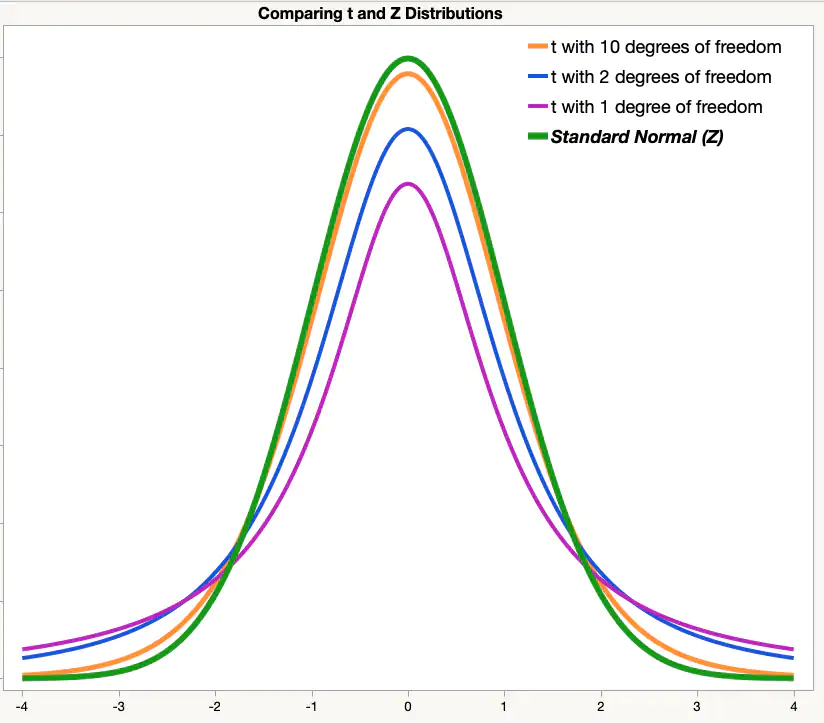
\includegraphics[width=0.6\textwidth]{fig/z-dist-and-t-dist.png}
    \caption{z分布与t分布的差异}
    \label{fig:z-and-t-dist}
\end{figure}

\subsubsection{两独立样本}

检验两个正态总体均值是否相等(Independent two-sample t-test)

【待补充】

\subsubsection{一元回归系数检验}

假设有如下线性回归模型,$x$已知,$\alpha$与$\beta$为待估参数,且$\epsilon$服从均值为0,方差未知假设为$\sigma^2$的正态分布:
\begin{equation*}
    y = \alpha + \beta x + \epsilon
\end{equation*}

此时检验回归系数$\beta$是否等于某$\beta_0$,一般假设$\beta_0 = 0$,即原假设为$X$与$Y$两者不存在线性关系。t-统计量(或t-score)服从自由度为$n-2$的t分布:
\begin{equation*}
    t\text{-statistic} = \frac{\hat{\beta} - \beta_0}{SE(\hat{\beta})} \sim T_{n-2}
\end{equation*}

其中有$\hat{\beta}$的标准误为:
\begin{equation*}
    SE_{\hat{\beta}} = \frac{\sqrt{\frac{1}{n-2} \sum_{i=1}^{n} (y_i - \hat{y}_i)^2}}{\sqrt{\sum_{i=1}^{n} (x_i - \bar{x})^2}}
\end{equation*}

对于残差,有:
\begin{equation*}
    \hat{\epsilon}_i = y_i - \hat{y}_i = y_i - (\hat{\alpha} + \hat{\beta} x_i )
\end{equation*}

由于残差平方和(Sum of squared residuals)为$SSR=\sum_{i=1}^n \epsilon_i^2$,可改写t-统计量为:
\begin{equation*}
    t\text{-statistic} = \frac{(\hat{\beta} - \beta_0)\sqrt{n-2}}{\sqrt{\frac{SSR}{\sum_{i=1}^{n} (x_i - \bar{x})^2}}}
\end{equation*}

\subsubsection{多元线性回归系数}

检验在多元线性回归中,$x_1,x_2,\dots,x_m$是否存在线性关系:

\begin{equation*}
    H_0: \beta_i = 0, \quad i=1,2,\dots,m
\end{equation*}

\subsection{F检验}

F检验(F-test)检验两个正态总体之间的方差是否相等,两个样本服从正态分布。

判断两组数据是否存在显著差异

F统计量为两个方差的比率:
\begin{gather*}
    F = \frac{\text{explained variance}}{\text{unexplained variance}} \\
    F = \frac{\text{between-group variability}}{\text{within-group variability}} 
\end{gather*}

具体而言,$S_1$与$S_2$为独立随机变量,且服从$\chi^2$分布,那么自由度为$\nu_1$与$\nu_2$的服从F分布的随机变量$F$为:
\begin{equation*}
    F = \frac{S_1/\nu_1}{S_2/\nu_2}
\end{equation*}

F分布的概率密度函数为,注意有$x\geq 0$,因为其为两个方差的比率:
\begin{equation*}
    f(x) = \frac{\Gamma\left(\frac{\nu_1+\nu_2}{2}\right)\left(\frac{\nu_1}{\nu_2}\right)^{\frac{\nu_1}{2}} x^{\frac{\nu_1}{2}-1}}{\Gamma\left(\frac{\nu_1}{2}\right)\Gamma\left(\frac{\nu_2}{2}\right)\left(1+\frac{\nu_1}{\nu_2}x\right)^{\frac{\nu_1+\nu_2}{2}}} \quad \text{for}\; x\geq 0
\end{equation*}

F分布概率密度函数(PDF)如下图所述,为右偏(Right skew)或正偏(Postive skew)。当$\nu_2>2$时,期望有$\frac{\nu_2}{\nu_2 -2}$。
\begin{figure}[ht!]
    \centering
    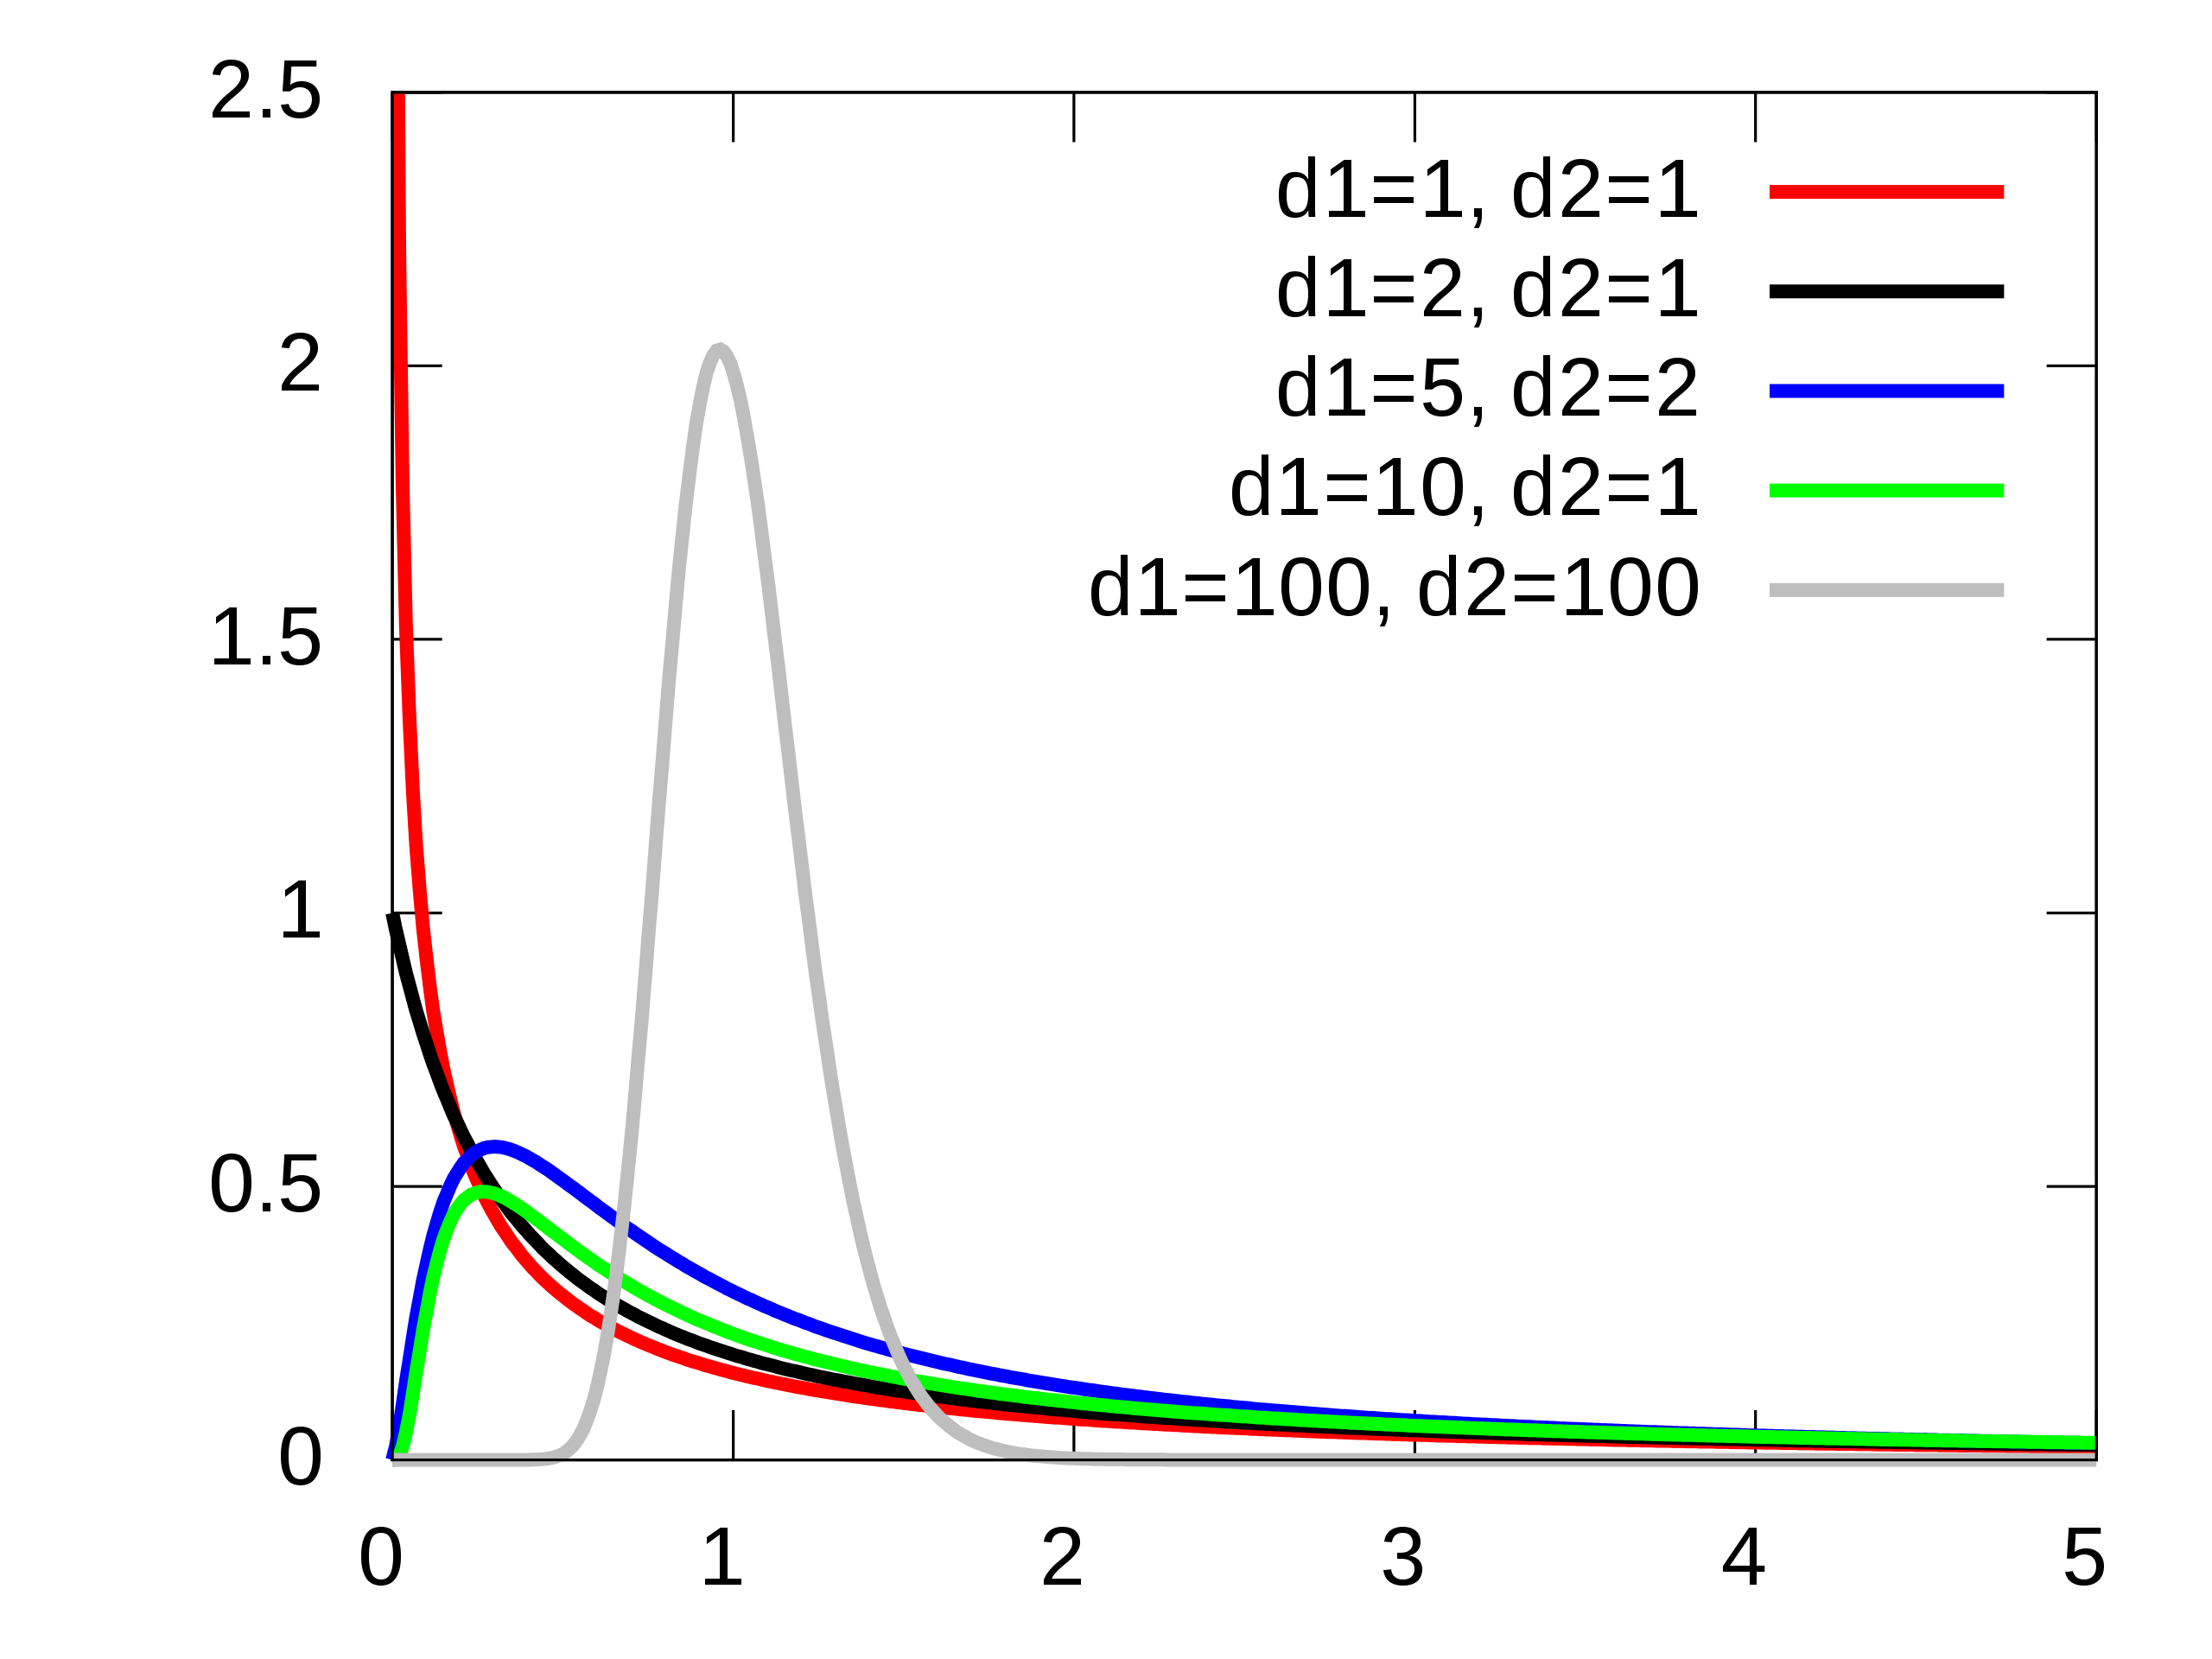
\includegraphics[width=0.8\textwidth]{fig/f-dist.png}
    \caption{F分布PDF}
    \label{fig:f-dist}
\end{figure}

检验变量$y$与$x_1,x_2,\dots,x_m$是否存在线性关系:
\begin{equation*}
    H_0: \beta_1 = \beta_2 = \dots = \beta_m = 0
\end{equation*}

$n$为样本数,$K$为变量数目,F统计量服从以自由度为$\nu_1=K-1$与$\nu_2=N-K$的F分布(查表用F-table)。
\begin{equation*}
    F-\text{statistic} \sim F_{K-1,N-K}
\end{equation*}

【待补充】

\subsection{\tops{$\chi^2$}检验}

卡方检验(Chi-squared test)为非参数检验,不存在具体参数和总体正态分布的假设。最初由统计天王Karl Pearson于1900年提出,是三大抽样(T检验、F检验与卡方检验)分布的检验里历史最悠久的。

卡方检验是比较数据的实测(实际观测值)分布与数的预期(理论预期值)分布的假设检验,检验两者之间的偏离程度,实际观测值与理论预期值之间的偏离程度就决定卡方的大小。如果卡方越大,二者偏差程度越大。相反,二者偏差越小。若两个值完全相等时,卡方值就为0,表明理论值完全符合。常见的卡方检验有:
\begin{itemize}
    \item 皮尔逊卡方检验(Pearson's chi squared test)
    \item 耶茨的连续性修正(Yates's correction for continuity)
    \item Fisher确切概率法(Fisher's exact test)
\end{itemize}

假设有随机变量$x_1,x_2,\dots,x_k$为独立随机变量,服从$N(0,1)$的标准正态分布。其令平方和为$Q$。则有$Q$服从自由度为$k>0$的卡方分布,即:
\begin{equation*}
    Q = \sum_{i=1}^{k} x_i^2 \qquad Q \sim \chi^2(k) \quad\text{or}\quad Q \sim \chi_k^2
\end{equation*}

对于自由度为$k$的卡方分布的概率密度函数(PDF)有:
\begin{equation*}
    f(x) = \frac{1}{2^{\frac{k}{2}}\Gamma\left(\frac{k}{2}\right)} x^{\frac{k}{2}-1} e^{-\frac{x}{2}}
\end{equation*}

卡方检验为单尾检验,拒绝域在右尾。当卡方分布的自由度$k<2$时,曲线呈现倒L形,当$k>2$时趋向于对称,而当$k\rightarrow \infty$时,则趋向于正态分布。
\begin{figure}[ht!]
    \centering
    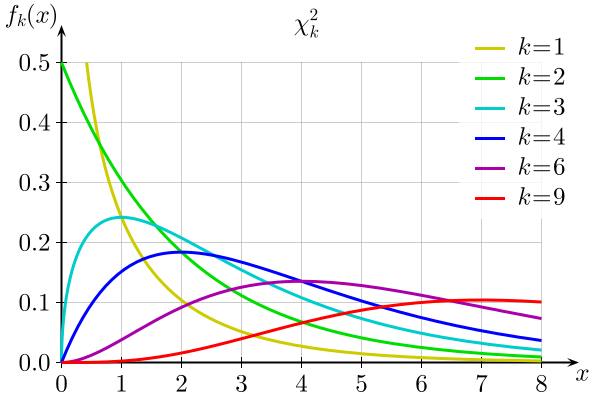
\includegraphics[width=0.8\textwidth]{fig/chi-squared.png}
    \caption{卡方分布PDF}
    \label{fig:chi-squared}
\end{figure}

\subsubsection{皮尔逊卡方检验}

皮尔逊卡方检验(Pearson's chi-squared test),当提及卡方检验,通常即指皮尔逊卡方检验。其中$O_i$指实际观察频数,$E_i$指理论预期频数:
\begin{equation*}
    \chi^2 = \sum_i^n \frac{(O_i - E_i)^2}{E_i}
\end{equation*}

皮尔逊卡方检验有多种用途:
\begin{itemize}
    \item 卡方拟合优度检验
    \begin{itemize}
        \item 使用此分析检验分类数据样本与总体理论分布的拟合程度
        \item 例如,通过多次掷骰子并使用卡方拟合优度检验来确定结果是否服从均匀分布,可以检验骰子是否公平。
    \end{itemize}
    \item 独立性和卡方检验
    \begin{itemize}
        \item 独立性检验:可以使用独立性检验确定一个变量的观测值是否取决于另一个变量的观测值。例如,确定某人投票的候选人是否与投票人的性别无关。
        \item 相关性检验:可以使用相关性检验确定一个变量是否与另一个变量关联。例如,确定不同颜色的汽车的销量是否取决于汽车售出的城市
    \end{itemize}
\end{itemize}

\subsubsection*{卡方拟合优度检验}
    
卡方拟合优度检验(Chi-square goodness of fit)或称拟合度的卡方检验、最佳拟合度卡方检验,用于检验实际数据是否符合理论分布,即度量实际分布与理论分布的拟合优度(Goodness of fit)。对于离散情形下,假设随机抽样的总样本量为$n$,分为互斥的$k$类,每一类的个体数为$x_i,\; i=1,2,\dots,k$为实际频数(个数),同时有$k$理论频数为,原假设为:
\begin{equation*}
    H_0: \text{第k类的占比为} p_i \quad i=1,2,\dots,k
\end{equation*}

此时有卡方统计量,分子为实际频数与理论频数的平方。服从自由度为$k-1$的卡方分布:
\begin{equation*}
    \chi^2 = \sum_{i=1}^{k} \frac{(x_i-np_i)^2}{np_i} \sim \chi^2(k-1)
\end{equation*}

\begin{example}
    孟德尔提出遗传第二定律,他发现有四种不同种类的豌豆种子:黄色圆形的、黄色褶皱的、绿色圆形的、绿色褶皱的。这些表现型类别(由可观察到的特征定义的类别)以大约9:3:3:1的比例出现。假设实际频数为315:108:101:32,总频数为556。那对于理论频数应有:
    \begin{equation*}
        556 \frac{9}{16} : 556 \frac{3}{16} : 556 \frac{3}{16} : 556 \frac{1}{16} = 312.75:104.25:104.25:34.75
    \end{equation*}

    因此计算卡方统计量有:
    \begin{equation*}
        \chi^2 = \frac{(315-312.75)^2}{312.75} + \frac{(108-104.25)^2}{104.25} + \frac{(101-104.25)^2}{104.25} + \frac{(32-34.75)^2}{34.75} = 0.47
    \end{equation*}

    对于显著性水平$alpha=0.05$,$\chi_(0.05,3)^2 = 7.815 > 0.47$,因此无法拒绝原假设,实验结果符合理论预期。
\end{example}

\subsubsection*{卡方独立性检验}

卡方独立性检验可用于判断两种因素是否独立,原假设为两种因素之间独立,而备择假设为两种因素之间非独立。

\begin{example}
    假设在赌场中,老板认为以为负责二十一点的庄家赔付的金额高于平均值,三位庄家观察的数据如下:
    \begin{table}[ht!]
    \centering
    \begin{tabular}{@{}ccccc@{}}
    \toprule
    & \textbf{庄家甲} & \textbf{庄家乙} & \textbf{庄家丙} & \textbf{合计} \\ \midrule
    \textbf{胜}  & 43 & 49 & 22 & 114 \\
    \textbf{平}  & 8 & 2 & 5 & 15 \\
    \textbf{负}  & 47 & 44 & 30 & 121 \\
    \textbf{合计} & 98 & 95 & 57 & 250 \\ \bottomrule
    \end{tabular}
    \end{table}

    此时原假设为庄家和赌局结果没有关系,而备择假设为有关系。对于庄家甲胜场的情况下,假设庄家与独具相互独立,应有理论频率为:
    \begin{align*}
        P(\text{庄家甲胜场}) &= \text{总场数} \times P(\text{庄家甲参加比例}) \times P(\text{胜场比例}) \\
        &= 250 \times \frac{114}{250} \times \frac{98}{250}
    \end{align*}

    计算所有理论频数为:
    \begin{table}[ht!]
    \centering
    \begin{tabular}{@{}cccc@{}}
    \toprule
    & \textbf{庄家A}& \textbf{庄家B} & \textbf{庄家C} \\ \midrule
    \textbf{胜} & $(114\times 98)/250$ & $(114\times 95)/250$ & $(114\times 57)/250$ \\
    \textbf{平} & $(15\times 98)/250$  & $(15\times 95)/250$  & $(15\times 57)/250$  \\
    \textbf{负} & $(121\times 98)/250$ & $(121\times 95)250$  & $(121\times 57)/250$ \\ \bottomrule
    \end{tabular}
    \end{table}

    计算卡方统计量:
    \begin{equation*}
        \chi^2 = \sum_i^n \frac{(O_i - E_i)^2}{E_i} = 5.62
    \end{equation*}

    对于显著性水平$alpha=0.05$,$\chi_(0.05,4)^2 = 9.488 > 5.62 $,因此无法拒绝原假设,赌局的胜负与庄家没有关系。
\end{example}

\subsubsection{确切概率法}

确切概率法(Excat Test)最常见的为Fisher确切概率法或称为四格表概率直接计算法
为2x2卡方独立性(independence)检验 

同时还有二项检验(Binomial test),为2x1卡方(goodness of fit)检验

\subsubsection{方差检验}

卡方检验也可以用来检验样本方差与总体方差是否相等,假设总体服从正态分布。

 The test statistic T in this instance could be set to be the sum of squares about the sample mean, divided by the nominal value for the variance (i.e. the value to be tested as holding). Then T has a chi-squared distribution with n − 1 degrees of freedom. 

但由于总体方差一般未知,因此较少使用

【待补充】

\subsection{方差分析}

方差分析(Analysis of variance,ANOVA),可以用于一次性检验多个(两个或两个以上)总体的均值是否相等,而T检验弱面对多个总体,只能两两进行比较。

\section{条件概率}

\subsection{条件概率}

条件概率(Conditional probability)记为$P(A\given B)$,指已知事件B发生的情况下事件A发生的概率,即把原本的样本空间,缩小为只有B发生的样本空间,从中再计算A发生的概率。而联合概率分布(Joint probability distribution)或简称为\textbf{联合分布},表示两个事件同时发生的概率,记为$P(A,B)$或$P(A\cap B)$,其样本空间为原本未缩小的空间。
\begin{equation*}
    P(A \given B) = \frac{P(A \cap B)}{P(B)}
\end{equation*}

\begin{remark}
    同理$P(B\given A) = \frac{P(A \cap B)}{P(A)}$,即有$P(A \cap B) = P(B\given A)P(A) = P(A\given B)P(B)$。易知同时满足AB条件的概率,即为已知满足A条件的子集中,再满足条件B的概率(为条件概率,即其样本空间为缩小后满足条件A的空间)。或满足条件B的子集中,再满足条件A的概率。
\end{remark}

\begin{example}
    假设有两个小碗,分别为甲碗与乙碗,每个小碗中有若干小球,共有蓝色与黄色两种颜色,具体数量如下。
    \begin{table}[ht!]
    \centering
    \begin{tabular}{cccc}\toprule
    & \textbf{蓝色} & \textbf{黄色} \\ \midrule
    \textbf{甲碗} & 1 & 4  \\
    \textbf{乙碗} & 3 & 2  \\ \bottomrule
    \end{tabular}
    \end{table}

    那么任意选取一个碗,并从中选取一个小球,颜色为蓝色的概率应为$P(\text{蓝色})=\frac{4}{10}$,同时有$P(\text{黄色})=\frac{6}{10}$。若已知取的碗为甲碗,那么选取蓝色小球的概率应为$P(\text{蓝色}\given \text{碗}=\text{甲碗})=\frac{1}{5}$,此时样本空间改变,被限制在了甲碗中,此时称为条件概率。

    若此时任意从两个碗中选取一个小球,小球颜色是蓝色,那么此时该小球是从甲碗中选取的概率为$P(\text{甲碗}\given \text{颜色}=\text{蓝色})=\frac{1}{4}$,注意$P(\text{甲碗}\given \text{蓝色})$与$P(\text{蓝色}\given \text{甲碗})$的概率并不相同。
\end{example}

\begin{example}
    假设某病患被检测出了某癌症阳性,该癌症在人群中的患病率(Prevalence)为$0.1\%$,并且该诊断的正确率为$99\%$。
    \begin{figure}[ht!]
    \centering
    \begin{tikzpicture}[
    grow = right, 
    level distance = 7em,
    level 1/.style={sibling distance=4.5em, anchor=west},
    level 2/.style={sibling distance=3em, anchor=west},
    ]
    \node {病患}
    child {
        node {不患癌症} 
        child {node {检测阴性} edge from parent node [above,sloped] {0.99}}
        child {node {检测阳性} edge from parent node [above,sloped] {0.01}}
        edge from parent node [above,sloped]{0.999}
    }
    child {
        node {患有癌症} 
        child {node {检测阴性} edge from parent node [above, sloped] {0.01}}
        child {node {检测阳性} edge from parent node [above,sloped] {0.99}}
        edge from parent node [above,sloped]{0.001}
    };
    \end{tikzpicture}
    \end{figure}

    该病人检测为阳性,因此有关的概率为$P(\text{患有癌症} \cap \text{检测阳性})$与$P(\text{不患癌症} \cap \text{检测阳性})$,而该病人在检测为阳性的前提下,真正患有癌症的概率应为:
    \begin{align*}
        P(\text{患有癌症}\given \text{检测阳性}) &= \frac{P(\text{患有癌症} \cap \text{检测阳性})}{P(\text{检测阳性})} \\
        &= \frac{P(\text{患有癌症} \cap \text{检测阳性})}{P(\text{患有癌症} \cap \text{检测阳性}) + P(\text{不患癌症} \cap \text{检测阳性})} \\
        &= \frac{0.001 \times 0.99}{0.001\times 0.99 + 0.999\times 0.01} \approx 9.016\% 
    \end{align*}

    或使用表格表示:
    \begin{table}[ht!]
    \centering
    \begin{tabular}{@{}lcc@{}} \toprule
    & 患有癌症(0.001) & 不患癌症(0.999) \\ \midrule
    检测正确($0.99$)& \textbf{检测结果:阳性} & 检测结果:阴性 \\
    检测错误($0.01$)& 检测结果:阴性 & \textbf{检测结果:阳性} \\ \bottomrule
    \end{tabular}
    \end{table}

    \begin{remark}
        在医学中将$P(\text{患病}\given \text{检测阳性})$的概率称为阳性预测值(Positive Predictive Value,PPV),即在检测为阳性的前提下,有多大概率是真正患病。具体为检测阳性并真实患病的人数(True Positve),除以全体检测阳性的人数。全体检测阳性的人数中,除了正确诊断的病患之外,还包含检测阳性但并不患病的人数(False Positve)。
        \begin{equation*}
            \text{PPV} = \frac{\text{TP}}{\text{TP}+\text{FP}}
        \end{equation*}
        
        如上所述,在医学中敏感性(Sensitivity)或真阳性率,指在病患中检测结果为阳性的概率。同样在病患中,检测为阴性的概率称为假阴性率,或漏诊率。而特异性(Specificity)或真阴性率,指在健康人群检测为阴性的概率。同样,在健康人群中,检测出阳性的概率称为假阳性率,或误诊率。
    \end{remark}
\end{example}

\subsection{条件概率分布}

继续推广条件概率的概念,条件概率分布(Conditional probability distribution),在离散形势下有称为条件概率质量函数(Conditional probability mass function):
\begin{equation*}
    P(X=x\given Y=y) = \frac{P(X=x\cap Y=y)}{P(Y=y)}
\end{equation*}

与条件概率相同,有等价关系$P(Y=y\given X=x)P(X=x) = P\left[(X=x)\cap (Y=y)\right] = P(X=x\given Y=y)P(Y=y)$。

\begin{example}
    有一个骰子,假设当掷出来的数字为偶数(如:$2,4,6$)时$X=1$,而奇数时$X=0$。同时假设当掷出来的数字为质数(如:$2,3,5$)时$Y=1$,其他情况下$Y=0$。
    \begin{table}[ht!]
    \centering
    \begin{tabular}{@{}ccccccc@{}}
    \toprule
    & \textbf{1} & \textbf{2} & \textbf{3} & \textbf{4} & \textbf{5} & \textbf{6} \\ \midrule
    \textbf{X} & 0 & 1 & 0 & 1 & 0 & 1 \\
    \textbf{Y} & 0 & 1 & 1 & 0 & 1 & 0 \\ \bottomrule
    \end{tabular}
    \end{table}
    
    对于无条件概率$P(X=1) = \frac{1}{2}$,而条件概率$P(X=1\given Y=1) = \frac{1}{3}$,具体计算如下:
    \begin{align*}
        P(X=1\given Y=1) &= \frac{P(X=1)P(Y=1\given X=1)}{P(Y=1)} \\
        &= \frac{P(X=1)P(Y=1\given X=1)}{P(X=1)P(Y=1\given X=1) + P(X=0)P(Y=1\given X=0)} \\
        &= \frac{1}{1+2} = \frac{1}{3}
    \end{align*}
\end{example}

对于连续情形下,有条件概率密度函数(Conditional probability density function):
\begin{equation*}
    f_{X\given Y}(x\given y) = \frac{f_{X,Y}(x,y)}{f_Y(y)}
\end{equation*}

如上所述其中$f_{X,Y}(x,y)$为联合分布(Joint probability distribution)。对于离散随机变量而言,称为联合分布概率质量函数(Joint probability mass function),对于连续随机变量也称为联合分布概率密度函数(joint probability density function)。而$f_Y(y)$为边缘分布(Marginal distribution),同样分为边缘概率质量函数(Marginal probability mass function)与边缘概率密度函数(Marginal probability density function)。

\subsubsection{链式法则}

对于概率论,同时也有链式法则(Chain rule)或称为一般乘法法则(General product rule),提供了使用条件概率分布计算联合概率分布的方法,如上所述对于时间$A$与事件$B$:
\begin{equation*}
    P(A\cap B) = P(A) \cdot P(B\given A)
\end{equation*}

对于多个事件$A_1,\dots,A_n$的联合分布,其中有$A_0$为全集,即$P(A_1\given A_0) = P(A_1)$:
\begin{align*}
    P(A_1 \cap \dots \cap A_n) &= P(A_1) \cdot P(A_2\given A_1) \cdot P(A_3\given A_2,A_1) \dots P(A_n\given A_{n-1},\dots,A_1) \\
    &= \prod_{i=1}^{n} P \left( A_i \:\left|\:\bigcap_{j=1}^{i-1} A_j \right. \right)
\end{align*}

如当$n=3$时,应有:
\begin{align*}
    P(A_1 \cap A_2 \cap A_3) &= P(A_3 \given A_2, A_1) \cdot P(A_2, A_1) \\
    &= P(A_3 \given A_2, A_1) \cdot P(A_2\given A_1) \cdot P(A_1)
\end{align*}

\subsubsection{条件期望}

与条件概率原理相同,条件期望(Conditional expectation),记为$\E(X\given Y)$或$\E(X\given Y=y)$,即限制条件$Y=y$缩小样本空间后,计算X的期望。在离散的情形下有如下表达式,其中$P(X=x,Y=y)$为联合概率密度函数。
\begin{equation*}
    \E(X\given Y=y) = \sum_x x P(X=x\given Y=y) = \sum_x x \frac{P(X=x,Y=y)}{P(Y=y)}
\end{equation*}

\begin{example}
    在上述投掷骰子的例子,对于无条件概率$\E(X) = \frac{1}{2}$,而条件期望$\E(X\given Y=1) = \frac{1+0+0}{3} = \frac{1}{3}$,条件期望$\E(X\given Y=0) = \frac{0+1+1}{3} = \frac{2}{3}$
\end{example}

对于连续随机变量,其中$f_{X,Y}(x,y)$为X与Y的联合概率密度函数,$f_Y(y)$为Y的概率密度函数,令$f_{X\given Y}(x\given y) = \frac{f_{X,Y}(x,y)}{f_Y(y)}$:
\begin{equation*}
    \E(X\given Y=y) = \int_x x f_{X\given Y}(x\given y) dx = \frac{1}{f_Y(y)} \int x f_{X,Y}(x,y) dx
\end{equation*}

\subsubsection{条件方差}

条件方差(Conditional variance)定义为:
\begin{align*}
    \Var(X\given Y) &= \E \left[\left( X-E(X\given Y) \right)^2 \given Y \right] \\
    &= \E \left[ X^2 - 2X\E(X\given Y) + \E^2(X\given Y) \given Y \right] \\
    &= \E (X^2\given Y) - \E^2(X\given Y)
\end{align*}

\begin{proposition}
    总期望定律(Law of total expectation)或称为双重期望定理(Double expectation theorem)有:
    \begin{equation*}
        \E(X) = \E\left[ \E(X\given Y) \right]
    \end{equation*}
    
    \begin{proof}
        \begin{align*}
            \E\left[ \E(X\given Y) \right]
            &= \sum_y \E(X\given Y=y) P(Y=y)\\
            &= \sum_y \left[ \sum_x x P(X=x\given Y=y) \right] P(Y=y) \\
            &= \sum_y \sum_x x P(X=x\given Y=y) P(Y=y) \\
            &= \sum_y \sum_x x P(Y=y\given X=x) P(X=x) \\
            &= \sum_x \sum_y x P(Y=y\given X=x) P(X=x) \\
            &= \sum_x x P(X=x) \left[ \sum_y P(Y=y\given X=x)\right] \\
            &= \sum_x x P(X=x) = \E(X)
        \end{align*}
    \end{proof}
\end{proposition}

\begin{remark}
    或可以先展开内层期望进行证明$\E\left[ \E(X\given Y) \right] = \E\left[ \sum_x x P(X=x\given Y) \right]$。由此可以发现内层条件期望求得的结果为关于Y的函数,因此外层的期望作用于随机变量Y,而内层的期望作用于随机变量X。积分先后顺序可以对调,可以理解为一个矩形面积,可以由积分底再积分高获得,或先积分高再积分底,两者结果相同。且倒数第二步,可以将与随机变量Y无关的,只关于随机变量X的部分提出至括弧外。
\end{remark}

\begin{proposition}
    总方差定律(Law of total variance)有:
    \begin{equation*}
        \Var(X) = \E\left[ \Var(X\given Y) \right] + \Var\left[ \E(X\given Y) \right]
    \end{equation*}

    \begin{proof}
        计算等式右边第一项,并且根据总期望定律:
        \begin{align*}
            \E[\Var(X\given Y)] &= \E\left[ \E(X^2\given Y) - \left( \E(X\given Y) \right)^2 \right] \\
            &= \E(X^2) - \E\left[ \left(\E(X\given Y)\right)^2 \right]
        \end{align*}

        对于等式右边第二项,根据方差的定义有:
        \begin{align*}
            \Var\left[\E(X\given Y)\right] &= \E \left[ \E(X\given Y) - \E\left[ \E(X\given Y) \right] \right]^2 \\
            &= \E \left[ \E(X\given Y) - \E(X) \right]^2 \\
            &= \E \left[ [\E(X\given Y)]^2 - 2\E(X\given Y)\E(X) + \E^2(X) \right] \\
            &= \E \left[ [\E(X\given Y)]^2 \right] - \E^2(X)
        \end{align*}
            
        将两项相加,再次根据方差定义$\Var(X) = \E(X^2) - \E^2(X)$替换,得证。
    \end{proof}
\end{proposition}

\subsection{贝叶斯定理}

通常而言,事件A在给定事件B已发生的条件下发生的概率,与事件B在给定事件A已发生的条件下发生的概率是不一样的。然而这两者是有确定的关系的,贝叶斯定理(Bayes' theorem)就是这种关系的陈述,具体而言有:
\begin{equation*}
    P(A\given B) = \frac{P(A)P(B\given A)}{P(B)}
\end{equation*}

$P(A)$为先验概率(Prior probability),即不考虑任何B方面的因素。而$P(A\given B)$为已知B发生后,A发生的概率,也称为A的后验概率(Posterior probability)或似然(Likelihood)。同理,所要求的条件概率$P(B\given A)$也称为B的后验概率,因为是在已知A发生的情况下,B发生的概率。

已知$P(A \cap B) = P(B\given A)P(A) = P(A\given B)P(B)$,由此变形可推导推导贝叶斯定理,即两个条件概率之间的关系。\textbf{注意}:只有当$A$与$B$互相独立时,才有$P(A \cap B) = P(A) \times P(B)$。由于此时$P(B\given A) = P(B)$,A不受B的影响。

\begin{example}
    继续使用小球的例子,并计算相应概率有:
    \begin{table}[ht!]
    \centering
    \begin{tabular}{cccc}\toprule
    & \text{蓝色(0.4)} & \text{黄色(0.6)} \\ \midrule
    \text{甲碗(0.5)} & 1 & 4  \\
    \text{乙碗(0.5)} & 3 & 2  \\ \bottomrule
    \end{tabular}
    \end{table}

    要计算$P(\text{甲碗}\given \text{蓝色})$,将样本空间限制在蓝色球的范围内,即应知道甲乙两个碗中蓝球的数目,最直观的计算方法为:
    \begin{equation*}
        P(\text{甲碗}\given \text{蓝色}) = \frac{P(\text{甲碗中蓝色球的数目})}{P(\text{甲碗中蓝色球的数目}) + P(\text{乙碗中蓝色球的数目})} 
    \end{equation*}

    其中分子甲碗中的蓝色球数目,应有甲碗的概率再乘以,已知甲碗蓝色球的概率(即在甲碗这个缩小的样本空间内,蓝色球的概率),若使用较为严谨的数学语音表达,则有:
    \begin{align*}
        P(\text{甲碗}\given \text{蓝色}) &= \frac{P(\text{甲碗})\times P(\text{蓝色}\given \text{甲碗})}{P(\text{甲碗}) \times P(\text{蓝色}\given \text{甲碗}) + P(\text{乙碗}) \times P(\text{蓝色}\given \text{乙碗})} \\
        &= \frac{P(\text{甲碗})\times P(\text{蓝色}\given \text{甲碗})}{P(\text{蓝色})} \\
        &= \frac{0.5 \times 0.2}{0.4} = \frac{1}{4}
    \end{align*}
\end{example}

\begin{example}
    上述癌症诊断例子中,患病率为$0.1\%$,并且该诊断的正确率为$99\%$。即在病患中检测出阳性的概率为真阳性率或敏感率为$99\%$,而在健康人群中检测为阴性的概率同为$99\%$,或称为真阴性率,或特异性。根据贝叶斯定理有:
    \begin{align*}
        P(\text{患有癌症}\given \text{检测阳性}) &= \frac{P(\text{患有癌症}) \times P(\text{检测阳性}\given \text{患有癌症})}{P(\text{检测阳性})} \\
        &= \frac{0.001 \times 0.99}{0.001\times 0.99 + 0.999\times 0.01} \approx 9.016\% 
    \end{align*}

    假设该病人进行了第二次同样的检测,此时再次使用贝叶斯定理,可以继续更新该病患真正患有癌症的概率,为了简便将条件事件$(\text{患有癌症}\given \text{第一次阳性})$记为$(\text{患癌首阳})$其概率近似为$9\%$代入计算。可以看到第二次检测阳性之后,实际患有癌症的几率大大提高。
    \begin{align*}
        &\hspace{1.6em} P(\text{患癌首阳}\given \text{第二次阳性}) 
        = \frac{P(\text{患癌首阳}) \times P(\text{第二次阳性}\given \text{患癌首阳})}{P(\text{第二次阳性})} \\
        &= \frac{P(\text{患癌首阳}) \times P(\text{第二次阳性}\given \text{患癌首阳})}{P(\text{患癌首阳})\times P(\text{第二次阳性}\given \text{患癌首阳})+ P(\lnot\text{患癌首阳}) \times P(\text{第二次阳性}\given \lnot\text{患癌首阳})} \\
        &= \frac{0.09 \times 0.99}{0.09\times 0.99 + 0.91\times 0.01} \approx 90.73\% 
    \end{align*}

\end{example}

\begin{remark}
    假设集合A为某假设或模型,而集合B为某事实或数据,那么有:
    \begin{equation*}
        P(\text{假设}\given \text{事实}) = \frac{P(\text{假设})P(\text{事实}\given \text{假设})}{P(\text{假设})P(\text{事实}\given \text{假设}) + P(\lnot \text{假设})P(\text{事实}\given \lnot \text{假设})}
    \end{equation*}
    
    贝叶斯定理可以通过图形进行理解与记忆,假设如下为边长为1的正方形,此时正方形面积为1代表整体概率为1。
    \begin{figure}[ht!]
    \centering
        \begin{tikzpicture}
            \draw (0, 0) rectangle (4, 4);
            \draw (1,0) -- (1,4);
            \draw (0,1.6) -- (1,1.6);
            \fill[pattern= north east lines] (0,0) rectangle (1,1.6);
            \draw (1,0.8) -- (4,0.8);
            \fill[pattern=north west lines] (1,0) rectangle (4,0.8);
            \draw[decorate,decoration={brace,amplitude=5pt,mirror,raise=0.2em}] (0,0) -- (1,0) node[midway,below,yshift=-0.6em]{\small $P(\text{假设})$};
            \draw[decorate,decoration={brace,amplitude=5pt,mirror,raise=0.2em}] (1,0) -- (4,0) node[midway,below,yshift=-0.6em]{\small $P(\lnot \text{假设})$};
            \draw[decorate,decoration={brace,amplitude=5pt,raise=0.2em}] (0,0) -- (0,1.6) node[midway,left,xshift=-0.6em]{\small $P(\text{事实}\given \text{假设})$};
            \draw[decorate,decoration={brace,amplitude=5pt,mirror,raise=0.2em}] (4,0) -- (4,0.8) node[midway,right,xshift=0.6em]{\small $P(\text{事实}\given \lnot \text{假设})$};
        \end{tikzpicture}
    \end{figure}

    假设$P(\text{假设})$不变,当$P(\text{事实}\given \text{假设}) = P(\text{事实}\given \lnot \text{假设})$时,即上图两个长方体高度相同。此时易知$P(\text{假设}\given \text{事实}) = P(\text{假设})$。此时,事实为真的概率,在假设条件为真与假设条件为假的两个子集中,概率相同,因此其概率就应该等于全样本下的先验概率,即后验概率不发生改变。由此可知,当事实为真的概率,在假设为真与假设为假的概率差别越大时,后验概率的变化也越大。
\end{remark}

\subsection{贝叶斯因子}

\subsubsection{后验因子估计}

关于贝叶斯定理,可以理解为根据已事实对认知进行更新。如在上述癌症诊断的例子中,原本的患病率为先验概率为$0.1\%$,通过已知的事实,原本的先验概率为后验概率,上升约为$9\%$。而这个上升的概率可以使用贝叶斯因子(Bayes factor)进行估算,是一种似然比(Likelihood ratio)。对于贝叶斯定理有:
\begin{equation*}
    \text{贝叶斯因子} = \frac{P(\text{事实}\given \text{假设})}{P(\text{事实}\given \lnot \text{假设})}
\end{equation*}

贝叶斯定理可以进行如下估算:
\begin{align*}
    P(\text{假设}\given \text{事实}) &= P(\text{假设})\times \frac{P(\text{事实}\given \text{假设})}{P(\text{事实})} \\
    &= P(\text{假设}) \times \frac{P(\text{事实}\given \text{假设})}{P(\text{假设})P(\text{事实}\given \text{假设}) + P(\lnot \text{假设})P(\text{事实}\given \lnot \text{假设})} \\
    &\approx P(\text{假设})\times \frac{P(\text{事实}\given \text{假设})}{P(\text{事实}\given \lnot \text{假设})} \\
    &= P(\text{假设})\times \text{贝叶斯因子}
\end{align*}

\begin{example}
    在上述癌症诊断例子中,患病率为$0.1\%$,并且该诊断的正确率为$99\%$。此时使用贝叶斯因子对后验概率进行估计:
    \begin{equation*}
        \frac{P(\text{检测阳性}\given \text{患有癌症})}{P(\text{检测阳性}\given \text{不患癌症})} = \frac{\text{True Postive Rate}}{\text{False Postive Rate}} = \frac{0.99}{0.01} = 99
    \end{equation*}

    因此$P(\text{患有癌症}\given \text{检测阳性}) \approx P(\text{患有癌症}) \times 99 = 0.1\% \times 99 = 9.9\% $,与实际计算结果$9.016\%$接近。此方法只在于帮助理解,贝叶斯定理实际上是一个更新概率的过程,实际的更新因子已由贝叶斯定理给出。由上式对比贝叶斯定理与贝叶斯因子估计,可以看出,当$P(\text{假设})$较小时,贝叶斯定理分母第一项趋近于0,此时$P(\lnot \text{假设})$趋近于1,使得两者较为接近。
\end{example}

\subsubsection{发生率与贝叶斯因子}

概率(Probability)与发生比(Odds)或俗称赔率的差别在于,就单一事件而言,概率中可包含多种结果,如上涨、不变、下跌,但发生率只能表示发生与不发生,两种结果。
概率的分子为单一结果,但分母是全体事件为1,而发生率分子与概率相同为单一结果,为发生,分母也为单一结果,即不发生。使得在发生率定义下,分母中不再包含$P(\text{假设})P(\text{事实}\given \text{假设})$项,使用贝叶斯因子能准确计算后验概率,而非估计,且形式更为简洁。

\begin{example}
    同样上述癌症诊断的例子中,患病率$0.1\%$转化为发生比为$1:999$,定义为先验发生比。此时贝叶斯因子的作用,是将分子患有癌症的人群中检测为阳性与分母中不患癌症中检测为阳性的人群分别挑选出来。因此结果就是检测为阳性的人群中,实际患有癌症的发生率。由上文计算贝叶斯因子为99,那么后验发生比为:
    \begin{align*}
        O(\text{患有癌症}\given \text{检测阳性}) &= \frac{\text{检测阳性且患有癌症的人数}}{\text{检测阳性但不患癌症的人数}} \\
        &= \frac{P(\text{患有癌症}) \times P(\text{检测阳性}\given \text{患有癌症})}{P(\text{不患癌症}) \times P(\text{检测阳性}\given \text{不患癌症})} \\
        &= O(\text{患有癌症}) \times \frac{P(\text{检测阳性}\given \text{患有癌症})}{P(\text{检测阳性}\given \text{不患癌症})} \\
        &= 1:999 \times 99 = 99:999 \\
        &\rightarrow \frac{99}{99+999} \approx 9.016\%
    \end{align*}
\end{example}

\section{似然}

对于似然(Likelihood)的简单理解,若已有数据$X$,想要猜测是来自分布$f$或分布$g$。那么将X的分布作图为直方图(Histogram),并同时对比两个分布,看分布$f$或分布$g$更为接近$X$的直方图,而似然就是对比的定量值。

对于数据集$X={x_1,x_2,\dots,x_n}$,并假设变量$x_i$均为独立同分布,即取值只与自己有关系,而与别的$x_j,j\neq i$无关。对于分布$f(\cdot \given \theta)$,对于任意$x_i$其概率$f(x_i \given \theta)$若非常低,则说明$x_i$出现在分布$f(\cdot \given \theta)$的概率非常低,而反之则说明概率高。即$x_i$有多大的可能性或概率,是来自分布$f(\cdot \given \theta)$,这其中的可能性或概率,即称之为似然。

\subsection{似然与概率}

如上所述,似然和概率,其本质都是可能性。对于由一组参数$\theta$确定的分布,概率是给定参数$\theta$,求某一结果的可能性。而相反而言,似然(Likelihood)是给定某一结果$X$,求参数$\theta$的可能性。具体而言,如对于只需要$\mu$与$\sigma$就能确定的正态分布,对于离散随机变量:
\begin{equation*}
    \mcl(\theta\given x) = P(X=x \given \theta)
\end{equation*}

对于连续随机变量:
\begin{equation*}
    \mcl(\theta\given x) = f(x\given \theta)
\end{equation*}

\begin{example}
    对于随机抽取实验室小白鼠,并测量其体重$w$的试验中,假设小白鼠的体重服从正态分布$N\sim(\mu,\sigma)$,此时概率为给定分布参数$\theta$的情况下,求小白鼠体重对应的概率:
    \begin{gather*}
        P( 32<w<34 \given \mu= 32,\sigma=2.5) = 0.29 \\
        P( w=34 \given \mu=34,\sigma=2.5) = 0.16
    \end{gather*}

    而对于似然,则为给定数据,求参数$\theta$对应的概率:
    \begin{gather*}
        L( \mu=32,\sigma=2.5 \given w=34) = 0.12 \\
        L( \mu=34,\sigma=2.5 \given w=34) = 0.21
    \end{gather*}

    在调整了分布的$\mu$之后,似然变大。显然对于单次的检验,单一数据,使得抽取一只小白鼠体重为$34g$的概率最大的分布,为$\mu=34$的正态分布。
\end{example}

\subsection{似然函数}

似然函数(Likelihood function)

\begin{equation*}
    \mcl(\theta \given X) = \prod_{i=1}^{n} f(x_i \given \theta)
\end{equation*}

\subsection{似然比}

似然比(Likelihood ratio)
\begin{equation*}
    \Lambda(\theta_1,\theta_2 \given x) = \frac{\mcl(\theta_1 \given x)}{\mcl(\theta_2 \given x)}
\end{equation*}

\begin{remark}
    在Python中有如下模块:
    \begin{itemize}
        \item \href{https://www.mathworks.com/help/econ/lratiotest.html}{Matlab: lratiotest}(Likelihood ratio检验)
    \end{itemize}
\end{remark}

\subsection{最大似然估计}
    
最大似然估计(Maximum likelihood estimation,MLE)

测量了数只老鼠的重量,尝试找到其分布,miximizes the likelihood 找到最大化所有观察重量likelihood的分布,找到mean 和standard deviation

\section{回归模型}

\subsection{回归模型分类}

\subsubsection*{线性回归模型}
线性回归模型(Linear regression)包含有:
\begin{itemize}
    \item 最小二乘法(Ordinary least squares)
    \item 广义最小二乘法(Generalized least squares)
    \item 加权最小二乘法(Weighted least squares)
    \item 广义线性模型(General linear model)
\end{itemize}

\subsubsection*{参数回归与半参数非参数回归}

参数回归或参数模型(Parametric regression),如各类线性回归,其回归函数形式为已知,参数待定,外延容易,但形式呆板。而对于半参或非参回归(Semi/Non-parametric regression),为非线性回归,其回归函数不确定,外延困难,但拟合效果却较好。其中非参数回归基本方法如:
\begin{itemize}
    \item 最近邻函数法(Nearest-neighbor或K-nearest neighbors)
    \item 核函数回归(Kernel regression)
    \item 神经网络(Neural networks)
    \item 支持向量机(Support vector regression)
    \item 光滑样条(Smoothing spline)
\end{itemize}

\section{时间序列}

\subsection{平稳性}

对于时间序列$\{r_t\}$,强平稳(Strongly stationary)或严格平稳(Strictly stationary),是指对于任意$t$和任意正整数$k$,资产收益率时间序列$(r_{t_1},\dots,r_{t_K})$与$(r_{t_1+t},\dots,r_{t_k+t})$的联合分布相同,即将$(t_1,\dots,t_k)$平移$t$个单位之后,分布不变。而弱平稳(Weakly stationary)指对于时间序列$\{r_t\}$,当$r_t$的均值与$r_{t-l}$的协方差不随时间改变,即:
\begin{gather*}
    \E [r_t] = \mu \\
    \Cov (r_t, r_{t-1}) = \gamma_l
\end{gather*}

$\mu$为常数,不随时间改变,而$\gamma_l$指依赖时间间距$l$的大小。平稳性的强弱区别,在于弱平稳只要求期望方差不变,即前两阶矩不变,而强平稳要求各阶距都不变。由于正态分布只需要两阶矩确认,因此时间序列$\{r_t\}$若是正态分布的,那么此时弱平稳与强平稳等价。

协方差$\gamma_l = \Cov(r_t,r_{t-l})$称为$r_t$的间隔为$l$的自协方差(Autocovariance),其中有两个性质:
\begin{gather*}
    \gamma_0 = \Var(r_t) \\
    \gamma_{-l} = \gamma_{l}
\end{gather*}

\begin{proof}
    性质二:
    \begin{equation*}
        \gamma_{-l} = \Cov(r_{t},r_{t-(-l)}) = \Cov(r_{t-(-l)},r_{t}) 
        = \Cov(r_{t+l)},r_{t}) = \Cov(r_{t)},r_{t-l}) = \gamma_{l}
    \end{equation*}
\end{proof}

\subsection{自相关函数}

\subsubsection{相关系数}

根据定义,两个随机变量$X$与$Y$的相关系数定义为:
\begin{equation*}
    \rho_{X,Y} = \frac{\Cov(X,Y)}{\sqrt{\Var(X)\Var(Y)}}
    = \frac{\E\left[(X-\mu_x)(Y-\mu_y)\right]}{\sqrt{\E(X-\mu_x)^2 \E(Y-\mu_y)^2}}
\end{equation*}

对于样本$\{(x_t,y_t)\}_{t=1}^{T}$,其中样本均值为$\bar{x}=\sum_{t=1}^{T}x_t/T$与$\bar{y}=\sum_{t=1}^{T}y_t/T$:
\begin{equation*}
    \hat{\rho}_{x_t,y_t} = \frac{\sum_{t=1}^{T}(x_t-\bar{x})(y_t-\bar{y})}{\sqrt{\sum_{t=1}^{T}(x_t-\bar{x})^2 \sum_{t=1}^{T}(y_t-\bar{y})^2}}
\end{equation*}

\subsubsection{自相关函数}

假设$\{r_t\}$为若平稳收益率时间序列,使用相关系数的概念推广至$r_t$与其过去值$r_{t-l}$,那么$r_t$与$r_{t}$的相关系数称为$r_t$间隔为$l$的自回归系数:
\begin{equation*}
    \rho_l = \frac{\Cov(r_t,r_{t-l})}{\sqrt{\Var(r_t)\Var(r_{t-l})}} 
    = \frac{\Cov(r_t,r_{t-l})}{\Var(r_t)}
    = \frac{\gamma_l}{\gamma_0}
\end{equation*}

由于$\{r_t\}$为弱平稳收益率时间序列,应有$\Var(r_t) = \Var(r_{t-l})$。根据定义,$\rho_0=1$且有$-1 \leq \rho_l \leq 1$。一个弱平稳序列,当且仅当对所有$l>0$都有$\rho_l=0$时,其为序列不相关。

对于$\{r_t\}$,其样本均值为$\bar{r}=\sum_{t=1}^{T}r_t/T$,间隔为l的样本自相关系数为:
\begin{equation*}
    \hat{\rho}_l = \frac{\sum_{t=l+1}^{T}(r_t-\bar{r})(r_{t-l}-\bar{r})}{\sum_{t=1}^{T}(r_t-\bar{r})^2} \qquad 0 \leq l < T-1
\end{equation*}

若$\{r_t\}$为\textbf{独立同分布}(i.i.d.)序列,满足$\E(r_t^2)<\infty$,那么对于任意正整数$l$,有$\hat{p}_l$渐进的服从均值为$0$、方差为$1/T$的$N\sim(0,\frac{1}{T})$的正态分布。

若$\{r_t\}$为\textbf{弱平稳}序列,满足$r_t = \mu \sum_{i=0}^{q}\phi_i a_{t-i}$,其中$\phi_0=1$,$\{a_i\}$为均值为0的独立同分布任意变量序列,对于$l>q$,则有$\hat{p}_l$渐进的服从如下正态分布,称为Bartlett公式:
\begin{equation*}
    \hat{p}_l \sim N\left(0,\frac{\left( 1+2\sum_{i=1}^{q}\rho_i^2 \right)}{T} \right)    
\end{equation*}

\subsubsection*{检验单个ACF}

对于正整数$l$,可以使用t检验(t-statistics)$t_{\hat{\beta}} = \frac{\hat{\beta}-\beta_0}{s.e.(\hat{\beta})}$来检验$H_0: \rho_l =0$与$H_a: \rho_l \neq 0$检验统计量为:
\begin{equation*}
    t_{\hat{\rho}} = \frac{\hat{\rho}_l}{\sqrt{\left( 1+2\sum_{i=1}^{q}\hat{\rho}_i^2 \right)/T}}
\end{equation*}

如果$\{r_t\}$为平稳的高斯序列并满足当$j>l$时,$\rho_j=0$,则有他检验渐进的服从\uline{标准正态分布}。此时为双侧检验,当$\abs{t_{\hat{\rho}}}>z_{\alpha/2}$时拒绝$H_0$,即在正态分布左右两端面积为$\alpha/2$的区域内拒绝$H_0$,而中间$1-\alpha$(置信水平)的区域不拒绝$H_0$。$Z_{\alpha/2}$为临界值(Critical value),临界值根据统计量的分布决定,由于统计量$t_{\hat{\rho}}$渐进服从标准正态分布,则此时具体为标准正态分布的$100(1-\alpha/2)$分位点。如此时$\alpha=5\%$,则有临界点为使得正态分布左侧阴影区域面积为$2.5\%$与$97.5\%$的两个$z$值,为$z=\pm 1.96$。


\divider

自相关(Autocorrelation)或称序列相关(Serial correlation)


自相关函数(Autocorrelation function,ACF)

The coefficient of correlation between two values in a time series is called the autocorrelation function (ACF), $Corr(x_t, x_{t-k}), k=1,2,3,\dotsc$




Durbin-Watson test

- H0: $\rho = 0$, no autocorrelation / serial correlation in residual
- H1: $\rho \neq 0$, autocorrelation in residual, follow first order autoregressive process

Test statistic
- resitual at lag 1, $\epsilon_t = \rho \epsilon_{t-1} + u_t$
- $DW = \frac{\sum_{t=2}^{T} (\epsilon_t - \epsilon_{t-1})^2}{\sum_{t=1}^{T} \epsilon^2_t}$

2 -> no autocorrelation
0-2 -> positive autocorrelation
2-4 -> negative autocorrelation

Ljung-Box test 

Test the null hypothesis that a series of residuals exhibits no autocorrelation for a fixed number of lags L. (See Box \& Pierce 1970, Q test)

- H0: No residual autocorrelation
- H1: There is residual autocorrelation

Test statistic

$$
Q = T(T+2) \sum^L_{k=1} \frac{\rho(k)^2}{T-k} > \chi^2_L
$$

- Q is chi-square with L degrees of freedom


\subsection{自回归模型}

自回归模型(Autoregressive model,AR)

向量自回归模型(Vector autoregressive model,VAR)
    
more than one random variable


\subsection{移动平均模型}
Moving-average (MA) model


\subsection{自回归移动平均模型}

自回归移动平均模型(Autoregressive moving-average model,ARMA)

\subsection{差分自回归移动平均模型}

差分自回归移动平均模型(Autoregressive integrated moving average,ARIMA)


\subsection{格兰杰因果关系}

格兰杰因果关系检验(Granger causality test)是一种假设检验的统计方法,检验一组时间序列x是否为另一组时间序列y的原因。它的基础是回归分析当中的自回归模型。


\subsection{单位根}

Dickey-Fuller test
H0: there is unit root, $\delta = \rho - 1 =0$, no stationary, random walk
H1: stationay, mean and variance do not change over time

A simple AR(1) model $y_t = \alpha + \rho y_{t-1} + u_t$, then we have $\Delta y_t = \alpha + (\rho -1) y_{t-1} + u_t = \alpha + \delta y_{t-1} + u_t$, 

Augmented Dickey-Fuller 

H0: there is unit root, $\delta = 0$
H1: stationary, $\delta < 0$

ADF test: $\Delta y_t = \alpha + \delta y_{t-1} + \beta_1 \Delta y_{t-1} + \cdots + \beta_{p} \Delta y_{t-p} + u_t$

AR(1) model: $\Delta y_t = \alpha + \delta y_{t-1} + u_t$
AR(2) model: $\Delta y_t = \alpha + \delta y_{t-1} + \beta \Delta y_{t-1} + u_t$

Test statistics: (negative, more negatvie -> reject H0)

-  $DF_{\delta} = \frac{\hat{\delta}}{SE(\hat{\delta})}$

ADF-Test: 检验结果为负,越负越拒绝原假设,即有单位根。单位根存在,即$y_t = a + b y_{t-1} + e_t$,$\abs{b} =1$,为随机。

\section{条件异方差模型}

\subsection{ARCH效应检验}

若将$a_t = r_t - \mu_t$为均值方程的残差,则可以用平方序列$a_t^2$来检验\textbf{条件异方差性},即所谓的ARCH效应。第一种方式,可以使用Ljung-Box统计量$\{Q(m)\}$应用于序列$\{a_t^2\}$,参见Mcleod和Li(1983)。该检验的原假设是$\{a_t^2\}$序列的前$m$个间隔的ACF值都为零。第二种方式,可以使用Engle(1982)中的拉格朗日乘子检验。

对于拉格朗日乘子检验(Lagrange Multiplier Test),等价于对如下线性回归中用F统计量检验$\alpha_i=0(i=1,\dots,m)$,即原假设有:
\begin{equation*}
    H_0: \alpha_1 = \dots = \alpha_m = 0
\end{equation*}

线性回归为:
\begin{equation*}
    a^2_t = \alpha_0 + \alpha_1 a^{2}_{t-1} + \dots + \alpha_m a^{2}_{t-m} + e_t \qquad t=m+1,\dots,T
\end{equation*}

$m$为正整数,$T$为样本容量,其中$e_t$为误差项,$\hat{e}_t$为上述线性回归最小二乘法估计的残差,$\bar{\omega}$为$a_t^2$的样本平均值。令:
\begin{gather*}
    SSR_0 = \sum_{t=m+1}^{T} (a_t^2 - \bar{\omega})^2 \qquad
    \bar{\omega} = \frac{1}{T} \sum_{t=1}^{T} a_t^2 \\
    SSR_1 = \sum_{t=m+1}^{T} \hat{e}_t^2
\end{gather*}

F统计量服从自由度为$m$的$\chi^2$分布,若$F>\chi_m^2(\alpha)$或F的p值小于$\alpha$则拒绝原假设,其中$\chi_m^2(\alpha)$为$\chi_m^2$上的$100(1-\alpha)$点:
\begin{equation*}
    F = \frac{(SSR_0-SSR_1)/m}{SSR_1/(T-2m-1)}
\end{equation*}

Ljung-Box Q-test
residual autocorrelation

Breusch–Godfrey test

test for autocorrelation in the errors in a regression model

Breusch–Pagan test

used to test for heteroskedasticity in a linear regression model

\begin{remark}
    ARCH效应检验或称为Engle's ARCH test,如上所述应平方序列检验异方差性,详情见Engle(1982),与其他检验如Ljung-box检验,拉格朗日检验,在Python与Matlab中有如下模块可进行计算:
    \begin{itemize}
        \item \href{https://www.statsmodels.org/stable/generated/statsmodels.stats.diagnostic.acorr_lm.html}{Python: acorr\_lm}(拉格朗日乘子序列相关检验)
        \item \href{https://www.statsmodels.org/stable/generated/statsmodels.stats.diagnostic.acorr\_ljungbox.html}{Python: acorr\_ljungbox}(Ljung-Box序列相关检验)
        \item \href{https://www.statsmodels.org/stable/generated/statsmodels.stats.diagnostic.het\_arch.html}{Python: het\_arch}(Engle异方差检验)
        \item \href{https://www.statsmodels.org/stable/generated/statsmodels.stats.diagnostic.het\_breuschpagan.html}{Python: het\_breuschpagan}(Breusch-Pagan拉格朗日乘子异方差检验)
        \item \href{https://www.mathworks.com/help/econ/lbqtest.html}{Matlab: lbqtest}(Ljung-Box序列相关检验)
        \item \href{https://www.mathworks.com/help/econ/archtest.html}{Matlab: archtest}(Engle异方差检验)
    \end{itemize}
\end{remark}

得分检验(Score test),score(informant) is the gradient of the log-likelihood function with respect to the parameter vetor.
\begin{equation*}
    s(\theta) = \frac{\partial \log \mcl(\theta)}{\partial \theta}
\end{equation*}

\begin{figure}[ht!]
    \centering
    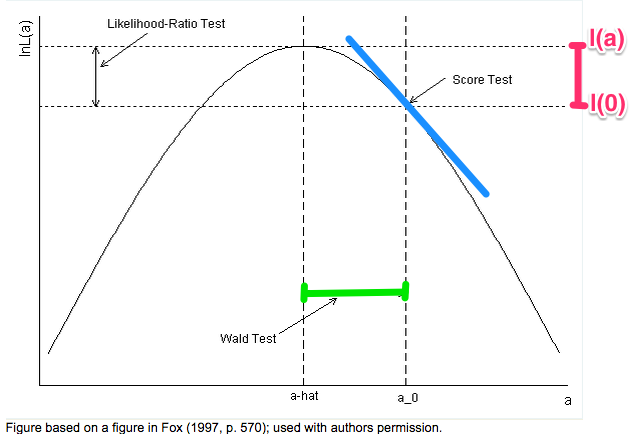
\includegraphics[width=0.8\textwidth]{fig/W-L-S-test.png}
    \caption{Likelihood/Wald/Score Test}
\end{figure}

\section{卡尔曼滤波}

卡尔曼滤波(Kalman Filter)的State Space Representation有:
\begin{align*}
   \mathbf{\xi_{t+1}} &= \mathbf{F \xi_{t}} + \mathbf{v_{t+1}} \\
   \mathbf{y_{t}} &= \mathbf{A'} \mathbf{x_{t}} + \mathbf{H'\xi_{t}} + \mathbf{w_t}
\end{align*}

定义有:
\begin{align*}
    \mathbf{P_{t\given t-1}} \equiv E[(\xi_{t} - \hat{\xi}_{t\given t-1})(\xi_{t} - \hat{\xi}_{t\given t-1})'] \\
    \mathbf{K_t} = \mathbf{FP_{t\given t-1}H(H'P_{t\given t-1}H+R)^{-1}}
\end{align*}

\begin{align*}
    E[(\xi_{t} - \hat{\xi}_{t\given t-1})(\xi_{t} - \hat{\xi}_{t\given t-1})'] &= \mathbf{P_{t\given t-1}} \\ E[(\mathbf{y_t} - \hat{\mathbf{y}}_{t\given t-1})(\mathbf{y_t} - \hat{\mathbf{y}}_{t\given t-1})'] &= \mathbf{H'P_{t\given t-1}H+R} \\
    E\{(\xi_t - \xi_{t\given t-1})(\mathbf{y_t} - \hat{\mathbf{y}}_{t\given t-1})'\} &= \mathbf{P_{t\given t-1}H} \\
\end{align*}

计算步骤
\begin{gather*}
    \hat{\xi}_{1\given 0} = E(\xi_1) \\
    P_{1\given 0} = E\{[\xi_1 - E(\xi_1)][\xi_1 - E(\xi_1)]'\}
\end{gather*}

迭代
% \begin{gather*}
%     \hat{\xi}_{t\given t} = \mathbf{\hat{\xi}_{t\given t-1} + P_{t\given t-1}H(H'P_{t\given t-1}H+R)^{-1}(y_t - A'x_t - H'\hat{\xi}_{t\given t-1})} \\
%     \hat{\xi}_{t+1\given t} = \mathbf{F \hat{\xi}}_{t\given t} = \mathbf{F\hat{\xi}_{t\given t-1} + K_t(y_t - A'x_t - H'\hat{\xi}_{t\given t-1})} \\
%     \mathbf{P}_{t\given t} = \mathbf{P_{t\given t-1} - P_{t\given t-1}H(H'P_{t\given t-1}H+R)^{-1}H'P_{t\given t-1}}
%     \mathbf{P}_{t+1\given t} = \mathbf{FP_{t\given t}F'+Q}
% \end{gather*}

平滑
\begin{gather*}
    \mathbf{J_t} \equiv \mathbf{P_{t\given t}F'P^{-1}_{t+1\given t}} \\
    \hat{\mathbf{\xi}_{t\given T}} = \hat{\mathbf{\xi}}_{t\given t} + J(\hat{\xi}_{t+1\given T} - \hat{\xi}_{t+1\given t})
\end{gather*}


\end{document}